\documentclass[10pt,journal]{IEEEtran}
%\documentclass{llncs}
%\documentclass[format=acmsmall]{acmart}
%\documentclass[sigconf]{acmart}
%\documentclass[sigconf,review, anonymous]{acmart}
\usepackage[noend]{algpseudocode}
\usepackage{standalone}
\usepackage{algorithm}
\usepackage{graphicx}
\usepackage{comment}
\usepackage{textcomp}
%\usepackage[dvipsnames]{xcolor}
\usepackage{color}
\usepackage{listings}
\usepackage{lstlinebgrd}
%\usepackage[compatibility=false]{caption}
\usepackage{balance}
\usepackage{wrapfig}
\usepackage{rotating}
\usepackage{amssymb}
\usepackage{amsmath}
\usepackage{multirow}
\usepackage{threeparttable}
\usepackage{subcaption}
\usepackage{enumitem}
\usepackage{calc}
\usepackage{pifont}
\usepackage{soul}
\usepackage{booktabs} % for \specialrule command, thick table line
\usepackage{cite}

\definecolor{pblue}{rgb}{0.13,0.13,1}
\definecolor{pgreen}{rgb}{0,0.5,0}
\definecolor{pred}{rgb}{0.9,0,0}
\definecolor{pgrey}{rgb}{0.46,0.45,0.48}
\definecolor{ppurple}{RGB}{138,43,226}
\definecolor{highlight}{rgb}{0.88,0.88,0.66}

\newcommand{\commentbs}[1]{{\color{blue} BS: \sf (#1)}}
\newcommand{\commenthb}[1]{{\color{purple} HB: \sf
#1}}
\newcommand{\commentws}[1]{{\color{red} WS: \sf (#1)}}
\newcommand{\commentnm}[1]{{\color{brown} NM: \sf (#1)}}
\newcommand{\commentcs}[1]{{\color{orange} CS: \sf (#1)}}
\newcommand{\commentty}[1]{{\color{green} TY: \sf (#1)}}

%  \newcommand{\tym}[1]{{#1}}
\newcommand{\tym}[1]{{\color{red} \sf #1}}

\makeatletter
\newcommand\notsotiny{\@setfontsize\notsotiny\@vipt\@viipt}
\makeatother


\newcommand{\subB}{\vspace{3pt}\noindent\textbf}
\newcommand{\subI}{\vspace{3pt}\noindent\emph}

\definecolor{tcolor}{rgb}{0,0.65,0}
\definecolor{fcolor}{rgb}{0.8,0,0}

\newcommand{\tp}{\textcolor{tcolor}{$\text{\rlap{\checkmark}}\square$}}
\newcommand{\fp}{\textcolor{fcolor}{$\boxtimes$}}
\newcommand{\fn}{\textcolor{fcolor}{$\square$}}

\newcommand{\cmark}{\text{\ding{51}}}%
\newcommand{\xmark}{\text{\ding{55}}}%

\algrenewcommand\alglinenumber[1]{\tiny #1:}
\algnewcommand\algorithmicforeach{\textbf{for each}}
\algnewcommand\algorithmicin{\textbf{in}}
\algnewcommand{\LeftComment}[1]{\State\(\triangleright\) #1}
\algdef{S}[FOR]{ForEach}[1]{\algorithmicforeach\ #1\ \algorithmicdo}
\algdef{S}[FOR]{ForEachIn}[2]{\algorithmicforeach\ #1\ \algorithmicin\ #2\ \algorithmicdo}

%\def \@atitle{{\normalsize GAIND}{\small ROID}}
%\def \@approach{\textsc{GAINdroid}}
\def \@atitle{{\normalsize SAINT}{\small DROID}}
\def \@approach{\textsc{SAINTdroid}}
\def \apptotal {3,571}

\lstdefinelanguage{Kotlin}{
  comment=[l]{//},
  emph={delegate, filter, first, firstOrNull, forEach, lazy, map, mapNotNull, println, return@},
  keywords={abstract, actual, as, as?, break, by, class, companion, continue, data, do, dynamic, else, enum, expect, false, final, for, fun, get, if, import, in, interface, internal, is, null, object, override, package, private, public, return, set, super, suspend, this, throw, true, try, typealias, val, var, vararg, when, where, while},
  morecomment=[s]{/*}{*/},
  morestring=[b]",
  morestring=[s]{"""*}{*"""},
  ndkeywords={@Deprecated, @JvmField, @JvmName, @JvmOverloads, @JvmStatic, @JvmSynthetic, Array, Byte, Double, Float, Int, Integer, Iterable, Long, Runnable, Short, String},
  sensitive=true,
}

\begin{document}

%\title{\@approach: Automatic Detection of API-related Compatibility Issues in Android Applications}
%\title{\@approach: General Automated Incompatibility Notifier for Android Applications}
%\title{General Automated Incompatibility Detection for Android} 
\title{SAINTDroid: Scalable, Automated Incompatibility Detection for Android} 
%\title{Detecting and Mitigating Architectural Mismatch in Evolutionary Android Systems}

\maketitle

\begin{abstract}
With the ever-increasing popularity of mobile devices over
the last decade, mobile applications and the frameworks upon
which they are built frequently change, leading to a
confusing jumble of devices and applications utilizing
differing features even within the same framework. For
Android apps and devices---the largest such framework and
marketplace---mismatches between the version of the app API
installed on a device and the version targeted by the
developers of an app running on that device can lead to
run-time crashes, providing a poor user experience. In this
paper, we present \@approach, a new analysis approach that
automatically detects all types of mismatches to which an
app may be vulnerable across versions of the Android API it
declaratively supports. 
We applied \@approach to 3,590 real-world apps and compared the results of our analysis against the state-of-the-art techniques,
which corroborates that \@approach is up to 76\% more successful in detecting compatibility issues, while issuing significantly less (11-52\%) false alarms.
We also show that our approach, which gradually loads and analyzes classes as needed, remarkably outperforms the existing techniques in terms of scalability.
%We applied \@approach to 3,590 apps and compared the results of our analysis against state-of-the-art tools. The experimental results corroborate its ability to outperform the existing techniques in terms of both the number and type of mismatches correctly identified  as well as run-time performance of the analysis.  

\end{abstract}

%\keywords{Android compatibility, program analysis, software evolution}

%\maketitle

\begin{IEEEkeywords}
Android compatibility, program analysis, software evolution
\end{IEEEkeywords}

\section{Introduction}\label{sec-intro}
\sloppy
Android is the leading mobile operating system representing over 80\% of the
market share~\cite{androidmarketstatistics}. The meteoric rise of Android is
largely due to its vibrant app market~\cite{googleplayapps}, which currently
provisions nearly three million apps, with thousands added or updated on a
daily basis.  Android apps are developed using an application development
framework (ADF) that ensures apps devised by a wide variety of suppliers can
interoperate and coexist as long as they comply with the rules and
constraints imposed by the framework.  An ADF exposes well-defined application
programming interfaces (APIs) that manifest the set of extension points for
building the application-specific logic, setting it apart from traditional
software systems often realized as a monolithic, independent piece of code.

The Android ADF frequently evolves, with hundreds of releases from multiple
device vendors since 2010~\cite{AndroidReleases}.
Such rapid evolution leads to
incompatibilities in Android apps targeted to older
versions of the framework.  As a result, defects and vulnerabilities, especially
following ADF updates, continue to plague the dependability and security of
Android devices and apps~\cite{linares2014api,Update4}. A recent
study shows that 23\% of Android apps behave differently after a framework
update, and around 50\% of the Android updates have caused instability in previously working
apps and systems~\cite{Helppi2014}. This has been referred to as ``death on
update''~\cite{death1,death2,death3,death4,iOS,youtube}.
 As part of Android ADF version 6.0 (API-level 23), Google introduced a dynamic permission system.  
%Google introduced a dynamic permission system as part of Android ADF version 6.0 (API-level 23).  
Previously, the permission system was entirely static, with the user
granting all requested dangerous permissions at install
time.  The new permission system instead allows users to
grant or revoke permissions at
run-time~\cite{permissiongroups}.  This new system creates a
new class of permissions-related incompatibility~issues.

Recent research efforts have studied compatibility
issues~\cite{huang2018understanding,wei2016taming,wu2017measuring},
but existing detection techniques target only certain
types of APIs.  For example, Huang et
al.~\cite{huang2018understanding} only targets API
callback related to lifecycles; identifying them requires
significant manual labor~\cite{huang2018understanding}
and thorough inspection of incomplete
documentation~\cite{wu2017measuring}.  Furthermore,
none of the state-of-the-art techniques consider
incompatibilities due to the dynamic permission system.
The state-of-the-art compatibility detection techniques
also suffer from acknowledged frequent ``false alarms''
because of the coarse granularity at which they capture
API information.  The lack of proper support for
detecting compatibility issues can increase the time
needed to address such issues, often longer than six 
months~\cite{siliconangle}.
Finally, these techniques~\cite{huang2018understanding,he2018understanding} have been shown facing difficulties in handling large scale libraries, due to direct loading of the entire code base for analysis purposes.

%\commentty{what about scalability issues faced by existing work since high scalability is one of the contributions of GainDroid?}



%\sloppy In this paper, we present a \textbf{g}eneral, \textbf{a}utomated
\sloppy In this paper, we present a \textbf{s}calable, \textbf{a}utomated
\textbf{i}ncompatibility \textbf{n}o\textbf{t}ifier for Android, dubbed \@approach, which automatically 
%\sloppy In this paper, we present \@approach (\textbf{G}eneral, fully \textbf{A}utomated \textbf{I}ncompatibility \textbf{N}otifier for And\textbf{DROID}), which automatically %detects compatibility issues regarding the use of all Android APIs and the new runtime permissions system. \commentty{through static analysis?}
detects all types of API- and permission-induced mismatches.
Existing state-of-the-art compatibility detection techniques
require to either analyze the entire ADF codebase or manually model common compatibility callbacks of ADF classes, prior to detecting incompatibilities~\cite{huang2018understanding,lili2018cid,he2018understanding};
as such they face serious scalability issues that limit their abilities to detect complex types of incompatibilities. 
Different from all these techniques, \@approach overcomes such scalability issues by gradually loading and analyzing classes, wherein a reachability analysis is leveraged to stumble on all pertinent classes.


%Different from the state-of-the-art compatibility detection techniques that rely on the traditional compiler-based approaches for static analysis~\cite{huang2018understanding,lili2018cid}, \@approach takes a class loader-based analysis approach that gradually loads and analyzes classes, wherein a reachability analysis is leveraged to stumble on all pertinent classes. \@approach then analyzes the identified API call sites and their concomitant conditions to effectively detect compatibility issues regarding the use of all Android APIs and the new runtime permissions system.



%\@approach has several advantages over existing work. First, unlike prior techniques that focus on specific types of APIs, our approach has the potential to greatly increase the scope of analysis by automatically and effectively analyzing all of the APIs in an ADF version. Second, \@approach also analyzes platform code to uncover compatibility issues that exist within the framework; these issues cannot be detected by analyzing only the application code---an approach commonly taken by the state-of-the-art incompatibility detectors~\cite{huang2018understanding,linttips, lili2018cid}.
%\commentty{We need to revise the above sentence ---  ICSE reviewer 1 says CiD does not analyze only the application code.}
%Third, incrementally loading and analyzing classes allows our technique to be remarkably faster and more scalable than the state-of-the-art in compatibility detection.

%\textcolor{blue}{ \@approach has several advantages
%over existing work.  First, unlike prior techniques
%that focus on specific types of APIs, our approach has
%the potential to greatly increase the scope of analysis
%by automatically and effectively analyzing all of the
%APIs in an ADF version.  Second, incrementally loading
%and analyzing classes allows our technique to be
%remarkably faster and more scalable than the
%state-of-the-art in compatibility detection.  Third,
%\@approach holistically analyzes application and ADF in
%tandem by gradually loading and analyzing classes as
%needed during the compatibility analysis. \@approach
%analysis, thus, can seamlessly move between the
%application code and the ADF code during the
%compatibility analysis.  Whereas prior techniques first
%analyze the ADF code, the results of which are
%subsequently used to resolve the API
%usages~\cite{huang2018understanding,linttips,
%lili2018cid}.  }

\textcolor{red}{
\@approach has several advantages over existing work.
First, \@approach holistically analyzes application and
ADF in tandem by gradually loading and analyzing
classes as needed during the compatibility analysis.
\@approach analysis, thus, can seamlessly move between
the application code and the ADF code during the
compatibility analysis.  Whereas prior techniques first
analyze the ADF code, the results of which are
subsequently used to resolve the API
usages~\cite{huang2018understanding,linttips,
lili2018cid}. Second, by actually analyzing app and ADF
code, our approach has the potential to greatly
increase the scope of analysis by automatically and
effectively analyzing all code in the utilized APIs in
an ADF version.  Prior techniques only focus on
specific types of APIs.  Third, incrementally loading
and analyzing classes allows our technique to be
remarkably faster and more scalable than the
state-of-the-art in compatibility detection.  
}

Our evaluation of \@approach against the
state-of-the-art analysis techniques using thousands of
real-world Android apps indicates that 
%Our experiments indicate that 
\@approach is up to 76\% more successful in detecting
compatibility issues, while issuing significantly less
(11-52\%) false alarms.  It also successfully detects
permission-induced mismatches that cannot be even
detected by state-of-the-art techniques.  In addition,
\@approach is  up to 8.3 times (four times on average)
faster than the state-of-the art techniques. 


%\commentty{Can we put the actual numbers here? E.g., the improvement of incompatibility detection,  performance gain, etc.}
%in the context of real-world Android
%apps collected from variety of repositories have been very
%The results, among other things, corroborate its
%ability to outperform existing analysis techniques both by
%remarkably decreasing the number of false positives and by
%detecting new classes of incompatibilities.  
To summarize,
this paper makes the following contributions:
 
 
\begin{itemize}
%\vspace{-0.2cm}
%{\color{green} 
\item \textit{General API and permission-induced incompatibility detection algorithms}: We
introduce novel algorithms that automatically detect all types of API incompatibilities and misuses of runtime permission
APIs to which an app may be vulnerable across ADF~versions.


\item \textit{Scalable incompatibility detection approach}:
We introduce a scalable analysis approach that can incrementally
load and analyze classes to handle large scale libraries in 
detecting incompatibility issues. 
%}

\item \textit{Publicly available tool implementation}: We develop a fully~automated
technology, \@approach, that effectively realizes~our
compatibility detection approach. We make \@approach publicly available to the research and education~community~\cite{GainDroid}.



\item \textit{Experiments}: We present results from
experiments run on 3,590 real-world apps and benchmark
apps, corroborating \@approach's ability in (1)
effective compatibility analysis of Android apps,
reporting many issues undetected by the
state-of-the-art analysis techniques; and (2)
outperforming other tools in terms of scalability.

\end{itemize}

The rest of this paper is organized as follows.
Section~\ref{sec-background} illustrates various examples of
Android compatibility issues.  Section~\ref{sec-approach}
provides an overview of \@approach to effectively detect
compatibility issues.  Section~\ref{sec-eval} describes our 
empirical study, and
Section~\ref{sec-results} reports the results. Finally, the
paper concludes with a discussion of %performance benefits
current limitations, and an outline of the related
research and future work.
 



\lstset{ 
    numbers=left, 
    stepnumber=1, 
%    basicstyle=\tiny\ttfamily,
    %basicstyle=\scriptsize\ttfamily,
    basicstyle=\footnotesize\ttfamily,
    captionpos=b, 
    breaklines=true, 
    tabsize=1, 
    numbersep=5pt, 
    xleftmargin=0.5cm,
    keywordstyle=\color{pblue}\bfseries, 
    commentstyle=\color{pgreen}
}

\section{API and Permission-Induced Compatibility Issues}\label{sec-background}

To motivate the research and demonstrate the need for
mechanisms for incompatibility detection, this section
describes three types of Android compatibility issues,
which can lead to runtime app crashes.
Table~\ref{tab:api-mismatch} summarizes API- and
permission-induced compatibility issues.  We will later
show how \@approach helps effectively identify these
incompatibility scenarios.

%\begin{comment}
%In this section, we provide background information related to the Android API and motivate the need for a technique that can effectively identify general API compatibility issues. We also describe and illustrate three types of API and permission-related compatibility issues, summarized in Table \ref{tab:api-mismatch}.
%\end{comment}

\begin{table}[h!]
\centering
\caption{Three Types of Compatibility Issues in Android. \label{tab:api-mismatch}}
%\footnotesize{
%\small{
%\scriptsize{
%\tiny{
\notsotiny{
\begin{tabular*}{\linewidth}{l|c|c|c|c|l}
    \hline
    \hline    
    \multicolumn{1}{c}{}              &\multicolumn{1}{|c}{}    & \multicolumn{1}{|c}{}              & \multicolumn{1}{|c}{App}   & \multicolumn{1}{|c|}{Device}& \\
    \multicolumn{1}{c}{Mismatch type} &\multicolumn{1}{|c}{Abbr.}& \multicolumn{1}{|c}{Compatibility} & \multicolumn{1}{|c}{level} & \multicolumn{1}{|c|}{level} & Results in mismatch if... \\
    \hline \hline
    API invocation                    &API & Backward & \rlap{$\geq\alpha$}\phantom{$<23$} & \rlap{$<\alpha$}\phantom{$\geq23$}    &app invokes API method      \\
    {\it (App $\rightarrow$ Android)} &    & Forward  & \rlap{$<\alpha$}\phantom{$<23$}    & \rlap{$\geq\alpha$}\phantom{$\geq23$} &\mbox{}introduced/updated in $\alpha$ \\
    \hline
    API callback                      &APC & Backward & \rlap{$\geq\alpha$}\phantom{$<23$} & \rlap{$<\alpha$}\phantom{$\geq23$}    &app overrides API callback  \\
    {\it (Android $\rightarrow$ App)} &    & Forward  & \rlap{$<\alpha$}\phantom{$<23$}    & \rlap{$\geq\alpha$}\phantom{$\geq23$} &\mbox{}introduced/updated in $\alpha$ \\
    \hline  
    Permission-                       &PRM & \multirow{ 2}{*}{Forward} & $\geq23$                           & $\geq23$                              &app misuses runtime \\
    induced                            &    &    & $<23$                              & $\geq23$                              &\mbox{}permission checking          \\ 
    \hline
    \hline
\end{tabular*}
}
\end{table}


\subsection{Android API Background}

As of August 2018, there are 26 releases of the Android API, most recently
API level 28~\cite{introducingAndroid9}.  Each version contains new and
updated methods to help developers improve app performance, security,
and user-experience. In this work, we mainly refer to each release of
the Android API by its API level (e.g., 26) rather than the associated name 
(Oreo) or Android version number (8.0)~\cite{androidversions}. 
Google strongly recommends that developers specify the range of the API levels
their apps can support in the manifest or Gradle file by setting
three specific attributes: (1) {\tt minSdkVersion}, which specifies the lowest level of the API supported by the app; (2) {\tt targetSdkVersion}, which specifies the level of the API used during app development; and (3) {\tt maxSdkVersion}, which specifies the highest level of the
    API supported by the app.\footnote{According to the Google documentation, declaring this attribute is not
    recommended~\cite{sdkversions} but installing an older app on a newer device
    may still lead to unexpected behavior~\cite{Update4}.}

\begin{comment}
\begin{description}[labelindent=2em,leftmargin=!,labelwidth=\widthof{\bfseries The longest label}]
    \item [{\tt minSdkVersion}] The lowest level of the API supported by the app.

    \item [{\tt targetSdkVersion}] The level of the API used during app development.  

    \item [{\tt maxSdkVersion}] The highest level of the
    API supported by the app.\footnote{According to the Google documentation, declaring this attribute is not
    recommended~\cite{sdkversions} but installing an older app on a newer device
    may still lead to unexpected behavior~\cite{Update4}.}

\end{description}
\end{comment}    
    
\subsection{API Compatibility Issues}
\label{API Compatibility Issues}

Incompatible API levels can cause runtime crashes in
Android apps installed on a device running a different
level of the API than that targeted by the app. Changes
to the API are generally additive, so most such crashes
stem from a lack of {\it backward-compatibility}, where
an app targeting a higher API level is installed on a
device running a lower one \cite{sdkversions}. However,
despite Google's assurances, there may also be issues
with {\it forward-compatibility} when an app is run on
a device with a higher API level than the app's target.
If the app invokes a method or overrides a callback
introduced in a newer level of the API than that
supported by the device or removed in a newer level of
the API than targeted by the app, a mismatch arises
(the two red regions as shown in
Figure~\ref{fig:api-mismatch}), which could potentially
crash the app.
%\commentty{Need to clarify the overriding a callback will cause incompatibility, raised by ICSE reviewer1.}

\begin{figure}%{R}{0.5\columnwidth}
    \centering
%    \vspace{-1ex}
    %\captionsetup{font=scriptsize,margin=5mm}
    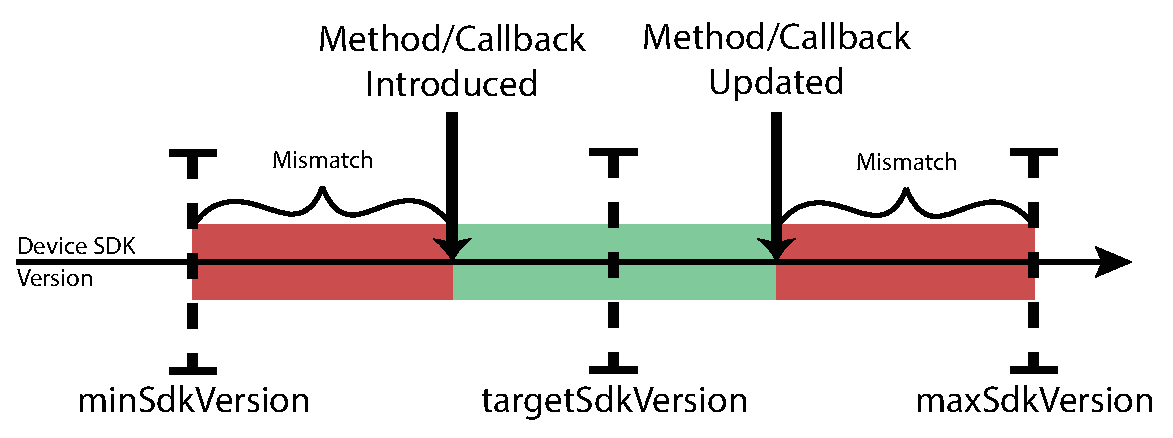
\includegraphics[width=0.85\columnwidth]{images/api-mismatch} 
    \vspace{-0.1cm}
    \caption{Mismatch between app and device API levels} 
    \label{fig:api-mismatch} 
    \vspace{-0.5cm}
\end{figure}

We divide these API incompatibilities into two types
(Table~\ref{tab:api-mismatch}): {\it invocation
mismatches}, where an app attempts to invoke an API
method not supported by the device; and {\it callback
mismatches}, where an app implements a callback method
missing from the API level installed on the device,
which will never be invoked.

%\vspace{-0.3cm}
\subsubsection{API invocation mismatch}

Mismatches in API method invocation occur when an app
developed against a higher version of the API attempts to
call a method introduced between its target version and that
installed on the device; the app crashes when the system
cannot find the desired method. Similarly, an app developed
against a lower version of the API may crash on a device
running a higher version if a method has been removed.
The former is an instance of a backward-compatibility issue, while the latter touches forward-compatibility, as referenced in Table~\ref{tab:api-mismatch}.

\begin{figure}[b]%[8]
%{R}{0.68\columnwidth}
    \vspace{-0.8cm}    
    \lstset{ 
        language=Java, 
        classoffset=1,
        morekeywords={activity_main, text, colorAccent}, 
        keywordstyle=\color{ppurple},
        classoffset=0, 
    } 
    %\vspace{-26pt}
    %\captionsetup{font=scriptsize,justification=centering}
    \lstinputlisting[ 
    caption={API Invocation Mismatch}, 
    label={lst:get-color-state-list},
    linebackgroundcolor={ 
        \ifnum \value{lstnumber}=9  \color{highlight} \fi
        \ifnum \value{lstnumber}=10 \color{highlight} \fi 
    } 
    ]{code_snippets/listing1.txt}
\end{figure}

 

Listing~\ref{lst:get-color-state-list} provides an illustrative example, where
the app targets Android API level 28, but its {\tt minSdkVersion} is set to 21.
In case the app is installed on a device with the Android API level 
21---the API level supported by the app according to 
its specified {\tt minSdkVersion}---it will crash on 
the invocation of {\sf getColorStateList}
(lines 9-10), which was introduced in API level 23.
One way to safeguard against this mismatch is to check the device's
API level at runtime, as shown in the comment on line 8.
This prevents the app from executing the call on versions
where it might be missing, but it is not fool-proof;
developers could easily forget to add or modify the check
when updating an app, leaving the code vulnerable to a
mismatch.


\begin{figure}%{R}{0.5\columnwidth} 
    \lstset{language=Java}
    \vspace{-0.7cm}       
    %\vspace{-31pt}
    %\captionsetup{font=scriptsize,justification=centering}
    \lstinputlisting[ 
    caption={API Callback Mismatch},
    label={lst:on-attach-context}, 
    linebackgroundcolor={ 
        \ifnum \value{lstnumber}=4 \color{highlight} \fi 
        \ifnum \value{lstnumber}=5 \color{highlight} \fi 
    }
    ]{code_snippets/callback-on-attach.txt} 
%    \vspace{-0.8cm}       
\end{figure}


%\vspace{-0.3cm}
\subsubsection{API callback mismatch}

API callback compatibility issues initiate in the Android system when its invokes callback methods overridden in the app.  Listing \ref{lst:on-attach-context} shows a snippet adapted from the \emph{Simple Solitaire}~\cite{simplesolitaire} app, where the API callback \textsf{onAttach(Context)}, which is introduced in API level 23, is overridden. The app is also specified to run on devices with API level lower than 23, which would not call that method. Thus, any critical actions (e.g., initialization of
an object) performed by the app in that method would be omitted, possibly
leading to runtime crashes. In the case where a callback is added to the API, this mismatch is a backward-compatibility issue; if a callback is removed, it is a problem with forward-compatibility.

\subsection{Permission-induced Compatibility Issues} \label{sec-background:prm}

With the release of Android API level 23 (Android 6), the
Android permission system is completely redesigned.  If a
device is running Android 5.1.1 (API level 22) or below, or
the app's {\tt targetSdkVersion} is 22 or lower, the system
grants all permissions at installation
time~\cite{permissiongroups}. On the other hand, for devices
running Android 6.0 (API level 23) or higher, or when the
app's {\tt targetSdkVersion} is 23 or higher, the app must
ask the user to grant dangerous permissions at runtime.  In
total, Android classifies 26 permissions as
dangerous~\cite{dangerousAPI}.  The goal of the new runtime
permission system is to encourage developers to help users
understand why an application requires the requested
dangerous permission~\cite{runtimepermissions}. 

\begin{figure}[b]%{R}{0.57\columnwidth} 
    \lstset{ 
        language=Java, 
        classoffset=1,
        morekeywords={activity_main, ACTION_IMAGE_CAPTURE},
        keywordstyle=\color{ppurple}, classoffset=0, 
    } 
    \vspace{-0.5cm}
%    \captionsetup{font=footnotesize}
    \lstinputlisting[
        caption={Permissions Mismatch (tgt $\geq$ 23)}, 
        label={lst:no-runtime-grant}, 
        linebackgroundcolor={ 
            \ifnum \value{lstnumber}=10 \color{highlight} \fi 
            \ifnum \value{lstnumber}=11 \color{highlight} \fi 
            \ifnum \value{lstnumber}=12 \color{highlight} \fi 
        }
    ]{code_snippets/listing3.txt} 
\end{figure}

Permission-induced incompatibility can also be divided into
two types of mismatch: {\it permission request mismatches},
where an app targeting API level 23 or higher does not
implement the new runtime permission checking; and {\it
permission revocation mismatches}, when an app targeting API
22 or earlier runs on a device with API 23 or later and the 
user revokes the use of a dangerous permission used by 
the app at runtime.
 
%\subsubsection{Permission request mismatch}

Listing~\ref{lst:no-runtime-grant} illustrates a permission
request mismatch; the app may crash on line 12 where it
attempts to use a dangerous permission it did not request.
To prevent the mismatch, the app would need to check the API
version and request permissions at runtime (shown as
comments on lines 7-9) and implement {\sf
onRequestPermissionsResult} (line 16). More detailed
examples of the new runtime permissions system can be seen
in the Android documentation \cite{runtimepermissions}.

%\subsubsection{Permission revocation mismatch}

If a user installs an app targeting APIs lower than 23 on a
device running API 23 or above, the user must accept all
dangerous permissions requested by the app at install time,
or the app will not be installed. However, API 23, 
i.e., Android version 6.0, allows the user to revoke those permissions
at any time. If the user revokes any dangerous permission in
the older app's setting after installation, the app would
crash while trying to use that permission--a permissions
revocation mismatch. This behavior has been recurrently
reported in real-world apps. \textit{AdAway}~\cite{adaway},
for example, tries to access external storage (such as an SD
card) at runtime. If that permission is revoked, the app
crashes when its tries to load data from the storage
mechanism.

\subsection{Limitations of Existing Work}


For existing incompatibility detection techniques to be able
to identify API and APC issues, they need to be able to
analyze both the application code and ADF code. Because the
ADF code can be very large, analyzing it would require a
significant amount of memory resource that may not be
feasible. Thus, a state-of-the-art technique, called
\textsc{Cider}~\cite{huang2018understanding}, conserves memory by creating models from the underlying ADF to represent API invocations and their
callback counterparts.  
As previously reported, creating models can be a daunting task
that may not be able to keep up with rapid releases of
ADFs~\cite{vanderMerwe2012}.  As will be shown later,
\textsc{Cider} can miss detecting compatibility issues that
exist in different ADFs.  Moreover, it is only capable of
detecting compatibility types that have been modeled.

%\textcolor{red}{
Another state-of-the-art incompatibility detector is
\textsc{CiD}\cite{lili2018cid}. This approach creates a
\emph{conditional call graph} for each app to record
method call information along with conditions checkers
related to API level. The construction of this graph is
done by performing an analysis path to identify API
calls. From each API call, \textsc{CiD} performs
backward data-flow analysis to identify the presence of
an API level check. Resolving API usage is then based
on the list of API calls and information from the
\emph{conditional call graph}.  To reduce memory usage,
\textsc{CiD} only analyzes the initial API call and
does not analyze subsequent calls within the
ADF~\cite{lili2018cid}.  As will be shown later, this
approach misses incompatibility issues that exist
deeper into the ADF code.  
%}

%\textcolor{red}{ 
Compared to \textsc{CiD}, our approach
gradually loads and analyzes classes from the
application code and ADF code.  For example, if an
application makes an API call, \@approach identifies
the class to which the invoked API belongs, then loads
just that class, and continues its analysis into that
class to detect the presence of API level checks and
any other issues that we wish to detect.  As such,
\@approach analysis can seamlessly 
%move between the application code and the ADF code,
%and 
produce a method-call graph that includes methods from
both app and ADF classes.  \@approach, therefore, can
achieve higher effectiveness to detect different types
of API compatibility issues. It also performs more
straightfoward analysis with fewer analysis passes,
resulting better memory conservation.  In the next
section, we describe the details of \@approach.  
%}



\section{Approach}\label{sec-approach}

%As previously mentioned, one major
%short-coming of the state-of-the-art approaches in
%detecting API compatibility issues is their inability
%to analyze application-under-analysis and the
%underlying ADF code in unison. As shown in
%Figure~\ref{fig:compare}a, these approaches perform
%analysis in two steps: analyzing the app and modeling
%the ADFs.  They then perform another layer of analysis
%that consider both results to detect API compatibility
%issues. In doing so, these approaches can miss
%detecting issues that lie deeper into the ADFs.   


 
\begin{comment}
\begin{figure}[t!]
    \centering
    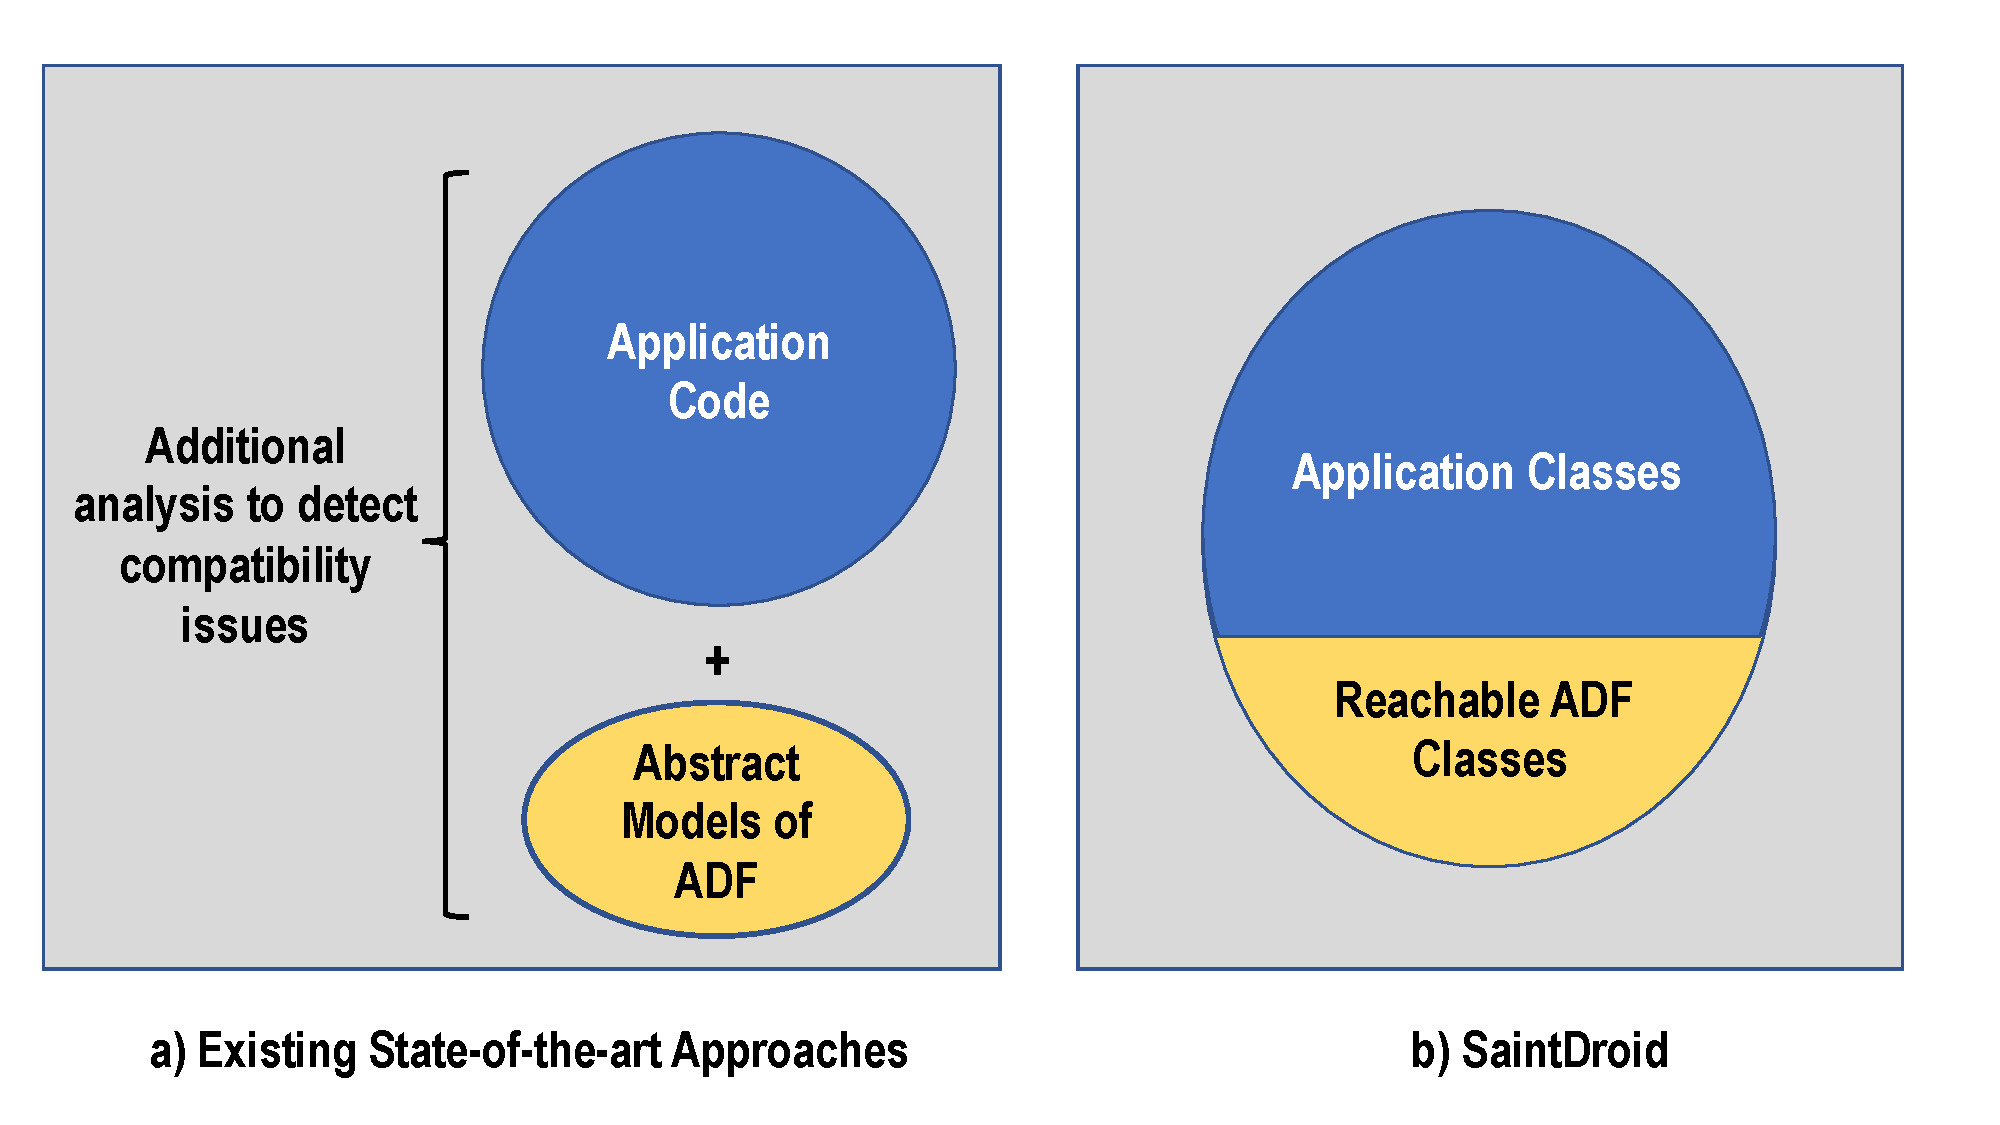
\includegraphics[width=\linewidth]{images/differences.pdf}
    %\vspace{-0.2cm}
    \caption{Comparing Existing Approaches with \@approach}
    \label{fig:compare}
    %\vspace{-0.3cm}
\end{figure}
\end{comment}

%\commentws{ \@approach can analyze the application and ADF code in unison by utilizing a novel class-loader-based program analysis approach. A class-loader is a runtime component that is part of any Java or Android Virtual Machine. It is responsible for incrementally loading any class needed during execution. It can accomplish this because of Java partition code into classes that can be individually loaded. \textit{\@approach adapts this runtime concept to support its scalable static analysis.} 


%In a nutshell, \@approach utilizes a \emph{ClassLoader Virtual Machine} (\emph{CLVM}) to perform class-based reachability analysis~\cite{tsutano2017efficient}. \emph{CLVM} takes advantage of code structure in Java to locate and load classes that can be reachable within a program.  As an example, if an application method calls an Android API, the class to which the API belongs would be loaded.  By utilizing CLVM, \@approach, as shown in Figure~\ref{fig:compare}b, analyzes the application classes and only the reachable ADF classes, and not the entire ADF code. This analysis approach blurs the line that separates application and ADF code and significantly reduces both peak memory footprint and memory consumption over time (as will be shown later). Currently, \@approach can only analyze Dex code; it does not support the loading and analysis of native code.  

This section overviews our approach to automatically detect all three types of API- and permission-induced mismatches. 
As depicted in Figure~\ref{fig:arch}, \@approach takes as input an app APK\footnote{APK is package containing byte code and other resources used to distribute and install an Android application.} along with a set of Android framework versions, and produces a list of mismatches for the given Android app.  
\@approach comprises two main components:
\begin{enumerate*}[label=(\arabic*)]
    \item The \textit{API usage modeler (AUM)} that utilizes different static analysis techniques, i.e., control flow and data flow analyses, to  identify the API call sites and the concomitant conditions thereof; and
    %\item The \textit{Android revision modeler (ARM)} that extracts essential information about the framework APIs' lifetime and mappings between Android API calls and the permissions required to perform those calls from the Android framework revision history;
    \item The \textit{Android mismatch detector (AMD)} leverages the artifacts produced by AUM to effectively detect API- and permission-related mismatches in the app under analysis.
\end{enumerate*}
%Next, we describe the details of each component in turn.
 

\begin{figure}[t!]
    \centering
%    %\vspace{0.2cm}
    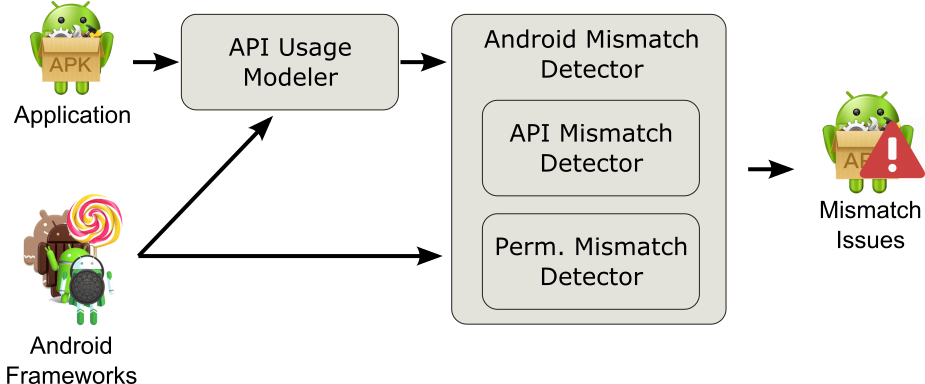
\includegraphics[width=0.8\linewidth]{images/Approach.png}
    %\vspace{-0.2cm}    
    \caption{Architecture of \@approach}
    \label{fig:arch}
    %\vspace{-0.6cm}
\end{figure}

\subsection{AUM: API Usage Modeler}
\label{API Usage Extraction}

The AUM module performs path sensitive, inter-procedural
data flow analysis on call and data flow graphs of a given
decompiled APK file to determine references to API methods
or callbacks.  More precisely, AUM derives an
inter-procedural control-flow graph, augmented to account
for implicit invocations (e.g., callbacks). The produced inter-procedural
control-flow graph is further annotated with permissions
required to enact Android API calls. Finally, a reachability
analysis is conducted over the augmented graph to identify
the guards that encompass the execution paths reaching the
annotated API calls or permission-required functionalities. 

\@approach's compatibility analysis has three major
advantages over the state-of-the-art approaches.
(1) To render our analysis more \emph{effective,
efficient, and scalable}, \@approach's AUM module
employs a novel class-loader based approach that incrementally discovers
pertinent application and ADF classes via reachability
analysis~\cite{tsutano2017efficient}.  
%It then analyzes only these classes. 
More specifically, \@approach's AUM module utilizes a \emph{Class Loader
Virtual Machine} (\emph{CLVM}) to perform class-based
reachability analysis~\cite{tsutano2017efficient}.
\emph{CLVM} takes advantage of the code structure in Java
to locate and load classes that can be reachable within
a program.  As a concrete example, if an application method
calls an Android API, the class to which the API
belongs would be loaded.  By utilizing CLVM, \@approach analyzes the application classes along with \emph{reachable} ADF classes, rather than analyzing the entire ADF codebase. 
%This analysis approach blurs the line that separates application and ADF code and significantly reduces both peak memory footprint and memory consumption over time.
This reduces both peak memory footprint and memory consumption over time, allowing \@approach
to be significantly faster and more space efficient
than the state-of-the-art in compatibility analysis.
The benefit comes without sacrificing the capability to detect
compatibility issues, as evidenced by the experimental
results (cf.  Section~\ref{sec-eval}).  
Some existing
state-of-the-art
techniques~\cite{huang2018understanding,he2018understanding},
on the other hand, directly load the entire code base
into memory, and thereby face scalability issues. 
%---\@approach's AUM module incrementally loads and analyzes
%classes 
(2) The AUM module analyzes actual ADF code to detect
\emph{more instances and types of compatibility issues}.
Prior work, on the other hand, focuses on creating models of
the ADF to only identify API callback compatibility
issues~\cite{huang2018understanding}.  
(3) While prior
work tends to analyze only the first call to the framework from an
app on each control flow path~\cite{lili2018cid}, the AUM module analyzes \emph{all} API calls and callbacks, which empowers
\@approach to detect \emph{more instances and types of
incompatibility issues}. 

\begin{comment}
Another key feature in Android that can affect the accuracy
of the compatibility analysis is late binding.  Indeed, apps
may dynamically load code that is not included in the main
dex file\footnote{A dex file incorporates compiled code which can be executed by an Android runtime.} of the
original application package, initially loaded at the
installation time.  This mechanism enables an app to be
extended with new desirable features at run-time. However,
in spite of its virtue, it poses challenges to analysis
techniques for assessing compatibility of Android apps.

To avoid missing any potential compatibility-related
issues that may result in crashes at run-time,
\@approach takes a conservative approach and considers
all possible bindings that can be statically
discovered.  More precisely, 
\end{comment}

Additionally, \@approach's AUM component
examines not only the main app code loaded at the
installation time, but also any other code accessible
from the app package that could be \emph{late bound}, or dynamically loaded, at run-time.
AUM incrementally augments the control-flow and
data-flow graphs by recursively identifying and
examining any classes which could be dynamically loaded by an app to
ensure that every method in every such class is
analyzed.\footnote{As one caveat, \@approach, as with any static analysis tool, cannot analyze classes dynamically loaded from remote servers.}
%Note that such to-be dynamically loaded code
%may not always be statically analyzable, especially
%when it is not bundled within installed packages, and
%rather externally loaded from remote servers.
  
  

\begin{figure}[t!]%{R}{0.66\textwidth}
%    \begin{minipage}{8cm}
        \begin{algorithm}[H]
%\footnotesize
	\small
	\begin{algorithmic}[1]
		\Procedure{FindApiMismatches}{block, app}\newline
		\Comment{{\bf Input:} Block from data flow graph, decompiled APK}
		\If{\Call{IsGuardStart}{block}}
		\State{(minLvl,maxLvl) $\gets$ \Call{GetGuard}{block,minLvl,maxLvl}}
		\ElsIf{\Call{IsApiCall}{block}}
		\ForEachIn{lvl}{(minLvl..maxLvl)}
		\If{$\neg$apidb.\Call{Contains}{block,lvl}}
		\State{mismatches $\gets$ mismatches $\cup$ \{block\}}
		\EndIf
		\EndFor
		\ElsIf{\Call{IsMethod}{block}}
		\State{mismatches $\gets$ mismatches $\cup$ FindApiIn(block, minLvl, maxLvl)}
		\ElsIf{\Call{IsGuardEnd}{block}}
		\State{(minLvl,maxLvl) $\gets$ (app.minSdk,app.maxSdk)}
		\EndIf
		\State{\Return{mismatches}}
		\EndProcedure
	\end{algorithmic}
	\captionof{algorithm}{Detecting API mismatches}
	\label{alg:api-mismatch}
\end{algorithm}
        %\vspace{-0.6cm}
%    \end{minipage}
\end{figure}

\begin{comment}
\subsection{ARM: Android Revision Modeler} 

The ARM module derives both the API lifecycle and the permission mapping models through mining of the Android framework revision history.
It first constructs an API database containing all public APIs defined in Android API levels 2 through 28\footnote{The Android frameworks range from API level 2 through API level 28, collected using {\it sdkmanager}, shipped with the Android SDK Tools to manage packages for the Android SDK~\cite{sdkmanager}. }, allowing \@approach to determine which methods and callbacks exist in each level within the app's supported range. \@approach automatically mines Android framework versions and stores the captured API information in a format that can be effectively queried by both the AMD module to generate the list of APIs in each level and a method call graph for each API method.
Note that the API database is constructed once for a given framework, i.e., an Android API level, as a reusable model upon which the compatibility analysis of all apps relies.
The Android revision modeling component to derive the lifetime of each framework's API is realized in an entirely automated fashion, which in turn facilitates supporting the upcoming versions of the framework. %\tym{Note that ARM differs from the API Lifecyle Modeling (ALM) component of CiD in the following ways: } \commentty{We should explicitly list the differences if there are any.}



 \@approach next extends the database with mappings between Android API methods and the permissions required by the Android framework during the execution of those methods. To achieve this, ARM relies in part on PScout~\cite{au2012pscout}, one of the most comprehensive permission maps available for the Android framework,%. The issue in using PScout was that its latest mapping was provided for the Android API level 22. ARM, therefore, 
 extended to include new mappings that would reflect more up to date Android API levels. Similar to the Android API database, permission maps are constructed once and reused in the subsequent analyses.
 

  

\end{comment} 
 
\subsection{AMD: Android Mismatch Detector} 
\label{mismatchdetection}

The AMD module analyzes the artifacts
produced by the AUM to identify
API-related invocation and callback mismatches ({\it API Mismatch Detector}) and permissions-related
mismatches ({\it Permissions Mismatch
Detector}).
%\subsubsection{API Mismatch Detector}\label{subsec-permission-identification}
%The \textit{Mismatch Detection} component first checks for API compatibility issues (cf.
%Section~\ref{API Compatibility Issues}), using the following process to spot both
%API invocation and callback mismatches:
 


\begin{figure}[t]
%    \begin{minipage}{8cm}
%        %\vspace{-1cm}
        %\begin{algorithm}[H]
%\scriptsize
\footnotesize
%\small
\begin{algorithmic}[1]
    \Procedure{IsApcMismatch}{method, app}\newline
    \Comment{{\bf Input:} Method from call graph, decompiled APK}
    \If {\Call{IsApiOverride}{method}}
        \ForEachIn{lvl}{(app.minSdk..app.maxSdk)}
            \If{$\neg$\Call{ApiContains}{method, lvl}}
                \State {mm $\gets$ mm $\cup$ \{method\}}
            \EndIf
        \EndFor
    \EndIf
    \State{\Return{mm}}
\EndProcedure
\end{algorithmic}
%\captionof{algorithm}{Detecting APC mismatches}
\caption{Detecting APC mismatches}
\label{alg:apc-mismatch}
%\end{algorithm}
        %\vspace{-3ex}
%    \end{minipage}
\end{figure}




\textit{Invocation mismatch:} The detector uses
the algorithm in Fig.~\ref{alg:api-mismatch} to detect API invocation
mismatches in each block of each method from the data flow
graph generated by static analysis of the app. If the
current block represents a guard condition (line 2), the
range of supported API levels is filtered by extracting the
minimum and maximum range from the guard and
updating the supported levels (line 3).
If the current block is a call to an API method (line 4),
check each supported API level to determine
whether the method called in the current block is defined in that level
(line 5-6).  In case that it is not defined, add the current
block to the set of mismatches (line 7).
%
In the case that an Android API is invoked inside a method
call, our algorithm (line 8) also checks if there is an
invocation to a user's defined method (i.e., not an
invocation to an Android API).  If this is the case, our
algorithm also analyzes the callee method  to look
for Android API invocations (line 9).
%This analysis process operates
%as a \emph{depth-first-search work-list} so it continues to
%follow any method invocation it encounters until reaching a
%terminal (i.e., a method that has no user defined method
%calls).
Finally, we reset the minimum and maximum supported
API levels to those defined in the app's manifest at the end
of each guard condition (lines 10-11).
%
%
%\commentws{Bruno, are you doing DFS with the algorithm? For
%example, if M1 is calling M2, then you would analyze M2 for
%API call. Let's say that in M2, there is a call to an
%Android API and then a call to M3, would you then go on and
%analyze M3? And if M3 calls M4, would your algorithm
%continues to analyze M4? Since you appears to be going
%deeper as more calls are encountered, I simply describe your
%algorithm as a DFS worklist. However, you will need to
%verify whether this is true.}
%
\@approach can reliably detect invocation mismatches because
the AUM component performs path-sensitive,
context-aware, and inter-procedural data-flow analysis,
which accounts for guard conditions on the
supported versions across methods, unlike other
state-of-the-art techniques, such as {\sc Lint} and {\sc
CiD}.



\begin{figure}[t!]%{R}{0.66\textwidth}
%    \begin{minipage}{8cm}
        %%\vspace{-5ex}
        \begin{algorithm}[H]%[t!] 
%\scriptsize 
%\footnotesize
\small
\relax 
%\caption{Detecting permission mismatches}
%\label{alg:permissions-mismatch}
\begin{algorithmic}[1]
\Procedure{DetectPermissionMismatch}{app, graph, permMap}
\newline\Comment{\rlap{\bf Input:}\phantom{\textbf{Output:}} Decompiled APK, call/data flow graph, permission map}
\newline\Comment{\textbf{Output:} List of detected mismatches}
    \State{dangerousPerms $\gets$ \Call{GetDangerousPermsFromManifest}{app}}
    \If{dangerousPerms $=\emptyset$}
        \State{\Return{$\emptyset$}}
    \EndIf
    \State{callGraph $\gets$ \Call{BuildCallGraph}{app}}
    \If{app.targetSdkVersion $\geq 23$}
        \ForEachIn{method}{callGraph}
            \If {\Call{OverridesOnRequestPermissionsResult}{method}}
                \State{\Return{$\emptyset$}}    
            \EndIf
        \EndFor
    \EndIf
    \State{mismatches $\gets\emptyset$}
    \ForEachIn{method}{callGraph}
        \State {dataFlowGraph $\gets$ \Call{GetDataFlowGraph}{graph, method}}
        \ForEachIn{block}{dataFlowGraph}
            \ForEachIn{perm}{dangerousPerms}
               	\If {permMap.\Call{IsUsingPermission}{perm, block}}
                   	\State{mismatches $\gets$ mismatches $\cup$ \{perm\}}
                \EndIf
            \EndFor
        \EndFor
    \EndFor
    \State{\Return{mismatches}}
\EndProcedure
\end{algorithmic}
\captionof{algorithm}{Detecting PRM mismatches}
\label{alg:prm-mismatch}
\end{algorithm}

 
%        %\vspace{-1cm}
%    \end{minipage}
\end{figure}

\textit{Callback mismatch:} %For each method in the call graph, the detector executes Algorithm~\ref{alg:apc-mismatch}. 
The detector uses the algorithm in Fig.~\ref{alg:apc-mismatch} to detect API callback mismatches in each method within the call graph derived from the app under analysis.
If the method overrides an API callback
(line 2), iterate over the API levels that the app declares to support and check whether the callback is defined within the entire range
of supported API levels (lines 4-5). This sets our approach apart from prior
research, such as {\sc Cider}~\cite{wu2017measuring}, through
\emph{automatically} detecting incompatible API callbacks without requiring any
manual effort of compiling a list of candidate callbacks beforehand, thereby
making it widely applicable and practical.





The second internal component of the AMD detects
incompatibilities surrounding the new runtime permissions system introduced in
API level 23, a capability unique to \@approach. %(outlined in Algorithm~\ref{alg:permissions-mismatch}).
The logic of the algorithm in Fig.~\ref{alg:prm-mismatch} that checks permission-induced compatibility issues is as follows:
First, extract dangerous permissions from the app's manifest (line 2).  
%If there are no
%dangerous permissions there is no risk of permission mismatches,
%as normal permissions are automatically granted (lines 3-4).  
In case the app
requests dangerous permissions, retrieve the call graph from the AUM component (line 5), and check whether each method of the app that
targets API level 23 or newer overrides {\sf onRequestPermissionsResult} (lines
6-8). In case the app does implement the new runtime permission system, there
is again no risk of mismatch (line 9).  If the app either does \emph{not} implement
the new runtime system \emph{or} targets an API level earlier than
23, each usage of a dangerous permissions could result in a mismatch and crash.
To detect dangerous permission usages, iterate through each method in the call
graph (line 11), retrieve the data flow graph for the method (line 12) and check
whether each block in the data flow graph uses any of the dangerous permissions
(lines 13-15). In case any dangerous permission is used, add it to the
set~of~mismatches~(line~16).




%\subsubsection{Permission Mismatch Detector}\label{subsec-permission-mismatch}


\def \apitotalALL {68,268}
\def \apctotalALL {2,115}

\def \apicountALL {1,471}
\def \apiprcntALL {41.19\%}
\def \apicountZOO {878}
\def \apicountFDR {593}

\def \apccountALL {761}
\def \apcprcntALL {20.05\%}
\def \apccountZOO {464}
\def \apccountFDR {252}

\def \andzooct {2,180}
\def \fdroidct {1,391}

\def \prqcount {224}
\def \prqprcnt {12.34\%}
\def \prqtotal {1,815}

\def \prvcount {1,206}
\def \prvprcnt {68.68\%}
\def \prvtotal {1,756}

\def \prmcount {1,430}
\def \prmprcnt {40.04\%}

\def \rqoneapps {19}

\section{Experimental Evaluation}
\label{sec-eval}

This section presents the experimental evaluation of~\@approach. 
%\textcolor{blue}{
We have implemented \@approach's static analysis capability on top of the \textsc{Jitana} framework~\cite{tsutano2017efficient}, %\textsc{Jitana} is a high-performance hybrid analysis tool for Android. It works directly on Dalvik executable (dex) files contained in each APK.
which is hybrid analysis tool for Android.
We also used \textsc{APKTool} \cite{apktool} for %reverse engineering Android APK files and 
extracting apps' manifest files.
As a result, our approach implementation only requires the availability of Android executable files, and not the original source code. \@approach, thus, can be used not only by developers, but also by end-users as well as third-party reviewers to assess the compatibility of their mobile apps.
%, which enables our tool to work on non-open source applications whose APKs can be found online. We also need to decompile the APK file to extract the manifest file, and to that end we use \textsc{APKTool} \cite{apktool}. 
%We further modified \textsc{Jitana} to decode dex files using Android version 6.0.0, which is the version in which the new runtime permissions system is introduced. We also extended \textsc{Jitana} to perform inter-procedural dataflow analysis, which enabled us to detect more API related issues within different methods of an Android app.
%}
\@approach's tool and the experimental data are available at the project website~\cite{GainDroid}.

We used the \@approach apparatus for carrying out the experiments. In our evaluation, we address the following research questions:

%Our evaluation of \@approach addresses the following research questions:

\textbf{RQ1.} \textit{Accuracy:} What is the overall accuracy of \@approach in detecting compatibility issues compared to the other state-of-the-art techniques?

\textbf{RQ2.} \textit{Applicability:} How well does \@approach perform in practice? Can it find compatibility issues in real-world applications?

\textbf{RQ3.} \textit{Performance:} What is the performance of \@approach's analysis to identify sources of compatibility issues?

\subsection{Objects of Analysis}

Our experimental objects are a set of Android apps
drawn from different sources.  

To evaluate the accuracy of our analysis technique and
compare it against the other compatibility analysis
tools, we used two suites of benchmark apps,
\textsc{CiD}-Bench~\cite{lili2018cid} and
\textsc{Cider}-Bench~\cite{huang2018understanding},
developed independently by other research groups.
%the DroidBench [4] and ICC-Bench [8] suites of
%benchmarks, two sets of Android applications
%containing ICC based privacy leaks for which all
%vulnerabilities are known in advance—establishing a
%ground truth.
%\commentty{The ICSE reviewer 1 noted that Cider did not evaluate recall, so he/she does not think \textsc{Cider}-Bench has ground truths. We should clarify.}
%
\textsc{CiD}-Bench contains seven benchmark apps and
\textsc{Cider}-Bench contains 20 apps.  The authors of
these benchmarks also reported known vulnerabilities.
We use these vulnerabilities as our evaluation
baseline. For example, we evaluate the effectiveness of
our approach by observing the number of reported
vulnerabilities in these two benchmarks that \@approach
can detect. If our approach detects a new issue, we
manually inspect whether the issue indeed exists.  
%
%\commentws{See above whether my explanation is sufficient.}
%We obtained seven benchmark apps from Li et
%al.~\cite{lili2018cid} and 20 apps from Huang et
%al.~\cite{huang2018understanding} as our objects of
%analysis, for which all compatibility issues are known
%in advance--establishing a ground truth.
The collection includes apps of varying sizes ranging
from 10,400 to 294,400 lines of Dex code and up to tens
of thousands of methods. The benchmark apps both
support and target a variety of API levels, with
minimum levels ranging from 10 to 21 and targets
ranging from level 23 to 27.  One of our baseline
system, i.e. \textsc{Lint}, requires building the apps
to perform the compatibility analysis. Out of the 27
benchmark apps, eight apps cannot be built\footnote{The
benchmark apps were built using Gradle~\cite{Gradle},
which dropped support of some Android SDK tool chains.
Even with the appropriate SDKs in place on two
different systems, Gradle were unable to build the
apps.}; therefore, they are excluded from the analysis,
leaving the total of \rqoneapps~apps used in
our~comparative~study.  Using the same benchmark apps
as prior research allows us to compare our results
against them and help eradicate internal threats to the
validity of our results.

To evaluate the implications of our tool in practice, we collected over 3,000 real-world Android apps from the following two sources:
%To further evaluate the applicability of our tool in practice, we collected a set of real-world Android apps from two repositories of FDroid~\cite{fdroid} and AndroZoo~\cite{allix2016androzoo}. 
(1) FDroid~\cite{fdroid} is a software
repository that contains free and open source Android
apps.  Our collection of subject systems includes all
\fdroidct\ apps available from the FDroid repository. 
(2) We also include 2,300 apps from AndroZoo~\cite{allix2016androzoo}, a growing repository of Android apps
collected from various sources, including the official Google Play store. We were
unable to build 120 of the apps from AndroZoo so we
excluded them from our analysis, leaving \apptotal~apps
in total.

\subsection{Variables and Measures}

\subB{Independent Variables.}
Our independent variables involve baseline techniques used
in our study to perform the analysis of compatibility issues.
These techniques include {\sc CiD}~\cite{lili2018cid}, {\sc
Cider}~\cite{huang2018understanding}, and
\textsc{Lint}~\cite{linttips}.

\textsc{CiD} represents a state-of-the-art in detecting
Android compatibility issues. It has been publicly released,
and we are able to obtain the tool and compile it in our
experimental environment.  We use it as the baseline system
to answer RQ1 and RQ3.

{\sc Cider} is another state-of-the-art approach developed to analyze API compatibility issues. Unfortunately, it is not available in  either source or binary forms at the
time of writing this article.  As such, we rely on their results as reported in \cite{huang2018understanding} to answer RQ1 and RQ3.

\textsc{Lint} is a static analysis technique, shipped
with the Android Development Tools (ADT), to examine
code bases for potential bugs, including incompatible
API usages.  \textsc{Lint} performs the compatibility
analysis as part of building apps, and thus requires the app source code to conduct the analysis. We use \textsc{Lint} to answer RQ1 and RQ3.

We also considered {\sc
IctApiFinder}~\cite{he2018understanding} as a possible
baseline technique. {\sc IctApiFinder} was introduced
at about the same time as \textsc{Cider}.
Unfortunately, the tool is not publicly available and
our attempts to contact the authors to request access
were unsuccessful. Therefore, we did not use it in our
study.

\subB{Dependent Variables.} As dependent variables, we chose
metrics allowing us to answer each of our three research
questions.

To measure accuracy, we compare the number of detected compatibility issues with known issues as reported by prior work~\cite{huang2018understanding,lili2018cid}. For each analysis technique, we report true and false positives and false
negatives thereof in detecting compatibility issues of the apps under analysis. Lastly, we report precision, recall and F-measure for each technique.


%We then report true (\tp) and false (\fp) positives and false negatives (\fn) based on comparisons to results from baseline techniques. Lastly, we report precision, recall and F-measure.


\newcommand{\timelbl}{Secs.}
%\begin{sidewaystable}
%\scriptsize
%\centering
%\begin{threeparttable}[c]
\begin{table}%[b!]
%\begin{tiny}
\caption {\label{tab:tab-results} Comparison between \@approach, \textsc{CiD}, \textsc{Cider}, and \textsc{Lint}. TP, FP and FN are~represented~by~symbols \tp, \fp, \fn, respectively. X(\#) indicates the number \# of detected instances for the~corresponding~symbol~X.}
%\vspace{-0.2cm}
%\small{
\scriptsize{
\begin{tabular}{l|ll|ll|ll} 
\hline
\hline
\rule{0pt}{3ex}
     & \multicolumn{2}{|c}{\sc \footnotesize{\@approach}} & \multicolumn{2}{|c}{\sc \footnotesize{CiD+Cider}} & \multicolumn{2}{|c}{\sc \footnotesize{Lint}} \\
 \multicolumn{1}{c|}{{\footnotesize App}} 
 & \multicolumn{1}{l}{API} & \multicolumn{1}{l|}{APC} 
 & \multicolumn{1}{l}{API} & \multicolumn{1}{l|}{APC} 
 & \multicolumn{1}{l}{API} & \multicolumn{1}{l}{APC} \\
\hline
\hline
\rule{0pt}{3ex}
 AFWall+         &  (\tp9)          & (\tp7)      & (\fn9)         & \tp(\fn6) &  \tp(\fn8) & (\fn7)          \\ 
 \midrule
 DuckDuckGo      &                  & \fn       & (\fp3)           & \tp         &               & \fn              \\ 
 \midrule
 \multirow{2}{*}{FOSS Browser}    &                  & \multirow{2}{*}{(\tp7)}   & \multirow{2}{*}{(\fp4)}       & \multirow{2}{*}{(\fn7)}     &  & (\fp3)  \\ 
    &                  &    &        &      &  & (\fn7)  \\ 
    \midrule
 \multirow{2}{*}{Kolab notes}     &  (\tp3)    &          & (\tp3)  & \multirow{2}{*}{\fp}        & \multirow{2}{*}{(\fn3)}       &              \\ 
      &  (\fp9)    &          & (\fp13)  &        &        &              \\ 
      \midrule
 \multirow{2}{*}{MaterialFBook}   &  (\tp11)&              & (\tp14)   &             & \multirow{2}{*}{(\fn14)}      &               \\
    &  \fp(\fn3)&              & (\fp17)   &             &       &               \\ 
    \midrule
 NetworkMonitor  &                  & (\tp5)  &                      & (\fn5)    &                 & (\fn5)            \\ 
 \midrule
 NyaaPantsu      &                  & (\tp12) &                       & (\fn12)   &   & (\fn12)          \\ 
 \midrule
 \multirow{2}{*}{Padland}         &                  & \multirow{2}{*}{\fn}     &      \multirow{2}{*}{(\fp4)}           & \multirow{2}{*}{\tp}       &  & (\fp2)         \\ 
          &                  &      &                 &        &  & \fn         \\ 
          \midrule
 PassAndroid     &  (\tp9)          & (\tp3)  &      (\fn9)          & (\fn3)      & (\fn9)       & (\fn3)            \\ 
 \midrule
 \multirow{2}{*}{SimpleSolitaire} &  \multirow{2}{*}{\tp\fp}          & \multirow{2}{*}{(\tp2)}  &      \tp       & \multirow{2}{*}{\tp\fn}      & \multirow{2}{*}{\fn}          & (\fp2)     \\
  &          &   &      (\fp10)       &       &          & (\fn2)     \\ 
  \midrule
 SurvivalManual  &                  &         &     (\fp19)        &           &  &                   \\ \midrule
 Uber ride       &                  & (\tp4)  &      (\fp2)         & (\tp4)     & & \fp(\fn4)    \\
\hline
\hline
 Basic       & \tp    & &  \tp        &  & \fn    &   \\ \midrule
 Forward     & \tp    &  & \tp        &  & \fn    &   \\ \midrule
 GenericType & \tp        & & \tp           &  & \fn       &   \\ \midrule
 Inheritance & (\tp2) &  & (\tp2)   &    & (\fn2) &   \\ \midrule
 Protection  &     &  &       &  &       &   \\ \midrule
 Protection2 &     &  &       &   & \fn    &   \\ \midrule
 Varargs     & (\tp2) &  & (\tp2)  &    & (\fn2) &   \\
\hline
\hline
\rule{0pt}{3ex}\textbf{Precision:} & \multicolumn{1}{l}{\bf 79\%} & \multicolumn{1}{l|}{\bf 100\%} &  \multicolumn{1}{l}{\bf  27\%} & 
 \multicolumn{1}{l|}{\bf 89\%} & \multicolumn{1}{l}{\bf 100\%} & \multicolumn{1}{l}{\bf 0\%} \\ 
{\bf Recall:}                   & \multicolumn{1}{l}{\bf 93\%} & \multicolumn{1}{l|}{\bf  95\%} &  \multicolumn{1}{l}{\bf 59\%} & 
\multicolumn{1}{l|}{\bf 19\%} &  \multicolumn{1}{l}{\bf 2\%} & \multicolumn{1}{l}{\bf 0\%}  \\ 
{\bf F-Measure:}                & \multicolumn{1}{l}{\bf 85\%} & \multicolumn{1}{l|}{\bf  98\%} & \multicolumn{1}{l}{\bf  42\%} & 
\multicolumn{1}{l|}{\bf 31\%} & \multicolumn{1}{l}{\bf 4\%} & \multicolumn{1}{l}{\bf 0\%}  \\ 
\hline
\hline
%\rule{0em}{3ex}
%\parbox[t]{5mm}{\multirow{4}{*}{\rotatebox[origin=c]{90}{AZ/FD\tnote{3}}}} & \multicolumn{13}{l}{\rlap{API}\phantom{PRM}$\rightarrow$\ \apitotalALL\ mismatches in \apicountALL\ apps (\apiprcntALL)} \\
%& \multicolumn{13}{l}{\rlap{APC}\phantom{PRM}$\rightarrow$\ \apctotalALL\ mismatches in \apccountALL\ apps (\apcprcntALL)} \\
%& \multicolumn{13}{l}{PRM$\rightarrow$\ \prmcount\ apps exhibiting mismatch (\prmprcnt)} \\
%& \multicolumn{13}{l}{\rlap{Time}\phantom{PRM}$\rightarrow$\ 6.6s / app on average (1.5s min, 16.8s max)} \\
%\hline
%\hline

\end{tabular}
% GD(API-I): pre=82.69%, rec=93.48%, f-measure=87.75%
% GC(API-C): pre=100%, rec=95.24%, f-measure=97.56%
% CiD: pre=21.11%, rec=95%, f-measure=42.85%
% CIDER: pre=88.89%, rec=19.05%, f-measure=31.38%
%\begin{tablenotes}
%\item[1]{\sc CiD} does not detect API callback mismatches.
%\item[2]{\sc Cider} does not detect API invocation or permissions-related mismatches and was not timed for RQ3.
%\item[3]{\apptotal\ apps from Androzoo and FDroid, analyzed with \@approach only.}
%\end{tablenotes}
%\end{threeparttable}
%\end{tiny}
}
%\vspace{-0.5cm}
\end{table}
%\end{sidewaystable}




To measure applicability, we report the number of detected
compatibility issues in real-world apps. Finally, to measure
performance, we report the analysis time and the amount of memory used by each of the analysis techniques, i.e., \@approach, {\sc CiD}, and \textsc{Lint}.


\subsection{Study Operation}

We conduct our experiments on a MacBook Pro running
High Sierra 10.13.3 with an Intel Core i5 2.5 GHz CPU
processor and 8 GB of main memory. To answer RQ1 and
RQ2, we run each analysis once since the techniques are
based on static analysis.  To handle uncontrollable
factors in our experiments addressing RQ3
(performance), we repeat the experiments three times
and measure the amount of time required to perform the
analysis of each app using the analysis techniques,
each averaged over three attempts. Further, since
\textsc{Lint} needs to build the app before it can
perform the analysis, we perform four consecutive
analysis attempts with {\sc Lint}, and report the
average analysis time of the last three analyses. 

%To answer RQ3, we measure the amount of time required to perform the analysis of each app using \@approach and {\sc CiD}, each averaged over three attempts.  \textsc{Lint} needs to build the app before it can perform the analysis, so we performed four consecutive analysis attempts with {\sc Lint}, and report the average analysis time of the last three analyses.

 
%\begin{comment}
\subsection{Threats to Validity}

The primary threat to external validity in this study
involves the object programs utilized. In this work,
we have studied a smaller set of benchmark programs
developed and released by prior research
work~\cite{lili2018cid,huang2018understanding} so that
we can directly compare our results with their
previously reported results.  However, we also extend
our evaluation to employ over 3,590 complex real-world apps from
other repositories, which in turn enabled us to assess our system in
real-world scenarios, representative of those that
engineers and analysts are facing.

The primary threat to internal validity involves
potential errors in the implementations of \@approach
and the infrastructure used to run \textsc{CiD} and
\@approach.  To limit these, we extensively validated
all of our tool components and scripts to ensure
correctness.  By using the same objects as our baseline
systems we can also compare the results produced by our
approach with those previously reported to help with
ensuring correctness.

The primary threat to construct validity relates to the
fact that we study efficiency measures relative to
applications of \@approach, but do not yet assess
whether the approach helps software engineers or
analysts addresses dependability and security concerns
more quickly than current approaches.
%\end{comment}



\section{Results and Analysis}
\label{sec-results}

%In this section, we report the results of our empirical evaluations to answer the three research questions.
 
%This section reports the data we collected to empirically address the three research questions, their interpretations, and our results.

\subsection{RQ1: Accuracy}


Table~\ref{tab:tab-results} summarizes the results of our
experiments for evaluating the accuracy of \@approach in
detecting compatibility issues compared to the other
state-of-the-art and state-of-the-practice techniques.  For
each app under analysis, we report the number of true (\tp)
and false (\fp) positives and false negatives (\fn)
according to the three categories of compatibility issues:

\textbf{API Invocation Compatibility Issues (API).}
\@approach succeeds in detecting all 8 known API
compatibility issues in \textsc{CiD}-Bench suite, and 33 API
compatibility issues out of 36 in \textsc{Cider}-Bench
suite.  It also correctly ignores 32 cases in \texttt{FOSS
Browser}, \texttt{Padland}, \texttt{DuckDuckGo},
\texttt{SurvivalManual} and \texttt{Uber~ride} apps, where
there are no API compatibility issues yet wrongly reported
by \textsc{CiD}. The only missed issues are the ones that
occur in the \texttt{MaterialFBook} app's anonymous classes,
not handled by our model extractor, discussed in more detail
in Section~\ref{sec-discussion}.  {\sc Cid} detects fewer
(26 out of 44) API invocation compatibility issues, and it has a high rate of
false positives, the majority of which arise because
\textsc{CiD}'s analysis is not context-sensitive and does
not track guard conditions across function calls.
\textsc{Lint} does even worse and only identified one of the
verified mismatches.  According to the results,
\textsc{Cider} is unable to examine Android apps for API
invocation compatibility issues. The results show that
\@approach outperforms the other three techniques in terms
of both precision and recall.


\textbf{API Callback Compatibility Issues (APC).} \@approach
successfully detects 40 callback compatibility issues out of
42 in the objects of analysis, with no false positives.
{\sc Cider} misses most of the issues identified by
\@approach mainly because it only considers the classes that
were manually modeled, i.e., {\sf Activity}, {\sf Fragment},
{\sf Service}, and {\sf WebView}. Whereas, \@approach
automatically identifies potential callback mismatches
across all classes in the Android API.  As expected,
\textsc{CiD} is unable to examine Android apps for callback
compatibility issues. \textsc{Lint} not only identifies none
of the verified mismatches, but also has a high rate of
false warnings. Overall, the results show that \@approach
outperforms the other three techniques in terms of both
precision and recall.


\textbf{Permission-induced Compatibility Issues (PRM).}
According to the experimental results, %shown in Table~\ref{tab:tab-results}, 
\@approach detects two cases of permission-induced compatibility issues in
\textit{FOSS Browser}~\cite{fossbrowser} and
\textit{Kolab notes}~\cite{kolab} apps; these two apps
request dangerous permissions and target an API level
higher than 23, yet they do not follow the new runtime
permission checking. Note that the other mismatch
detection techniques do not detect any of the runtime
permission compatibility issues.  Next, we evaluate
whether \@approach is sufficiently robust to handle
large real-world apps.


\subsection{RQ2: Real-World Applicability}

To evaluate the implications of our tool in practice, we applied \@approach to real-world apps collected from a variety of repositories (cf. Section~\ref{sec-eval}).
%When applied to real-world apps, 
\@approach detected 68,268 potential API invocation mismatches, with 41.19\% of the
apps harboring at least one potential mismatch. It also
identified 2,115 potential API callback mismatches occurring
in 20.05\% of the apps under analysis.  To perform the
permission-induced mismatch analysis, we divided the apps
into two groups based on the target SDK version: (i) 1,815
apps target Android API levels greater than or equal to 23
and (ii) 1,756 apps target Android API levels below 23. We
identified a total of 1,430 apps across both groups with at
least one permissions-induced compatibility issue. 224 apps
(12.34\%) in group (i) attempt to use dangerous permissions
without implementing the runtime permissions request system,
and 1,206 apps (68.68\%) in group (ii) are vulnerable to
permissions revocation mismatches (cf.
Section~\ref{sec-background:prm}).

%\commentty{added text below.}
Since manually examining all 3,691 real-world apps 
prohibitively expensive, we sampled 60 apps where 
incompatibilities were detected and calculated 
the precision scores. We do not consider
recall because the ground-truth incompatibilities
are unknown. Among all 60 incompatibility issues,
the precision scores for API invocation, callback, and permission
incompatibilities are 85\%, 100\%, and 100\%, respectively. 
The results are consistent with the ones obtained from the benchmark programs (cf. Table~\ref{tab:tab-results}). 

%Because the apps in group (i) are more recent, they are
%also representative of apps that are currently used on
%devices.  Therefore, we further investigate the usage
%of dangerous permissions among the apps in this group.
%After studying the apps, we realized that these apps
%only use 10 out of 26 dangerous
%permissions~\cite{dangerousAPI}. Within the group, 127
%apps, mostly targeting API level 23, requested these 10
%permissions. The permission WRITE\_EXTERNAL\_STORAGE is
%the most requested by applications (110 times),
%followed by READ\_EXTERNAL\_STORAGE (47 times) and
%READ\_PHONE\_STATE (31 times). Some dangerous
%permissions such as READ\_CALENDAR, WRITE\_CALENDAR and
%READ\_CONTACTS were not requested at all.
 
We then investigated the \@approach's results to
appraise its utility in practice. In the following, we
report some of our findings. To avoid revealing previously
unknown compatibility issues, we only disclose a subset of
those that we have had the opportunity to bring to the app
developers' attention.

%\commentty{where are the results below from? I assume they are not from the 68,268 apps? We should clarify}


%API invocation -> org.sufficientlysecure.localcalendar_9:

\textbf{API invocation mismatch.} In the \textsf{Offline
Calendar} app~\cite{offlinecalendar}, the invocation of the
\textsf{getFragmentManager()} API method in
\textsf{PreferencesActivity.onCreate} causes an API
invocation mismatch.  The \textsf{getFragmentManager()}
method was added to the \textsf{Activity} class in API level
11. Yet, \textsf{Offline Calendar} sets its
\textsf{minSdkVersion} to API level 8. Therefore, as soon as
the \textsf{PreferencesActivity} is activated, the
\textsf{Offline Calendar} app will crash if running on API
levels 8 to 11. The mismatch could be resolved by wrapping
the call to \textsf{getFragmentManager()} in a guard
condition to only execute it if the device's API level is
equal or greater than 11, or by setting the
\textsf{minSdkVersion} to 11.
%API callback -> be.digitalia.fosdem_1500150:

\textbf{API callback mismatch.} FOSDEM~\cite{fosdem} is a
conference companion app.  It exhibits an API callback
mismatch in its \textsf{ForegroundLinearLayout} class, which
overrides the \textsf{View.drawableHotspotChanged} callback
method, introduced in API level 21. However, its
\textsf{minSdkVersion} is set to API level 15, which would
not support the aforementioned callback method, and in turn
may not properly propagate the new hotspot location to the
\textsf{Drawable} stored as a member of the layout class.
This could lead to crashes or other instability in the app
interface. Setting the \textsf{minSdkVersion} to 21 would
resolve the mismatch.



%permission request mismatch -> org.kore.kolabnotes.android_98:

\textbf{Permission request mismatch.} \textsf{Kolab
Notes}~\cite{kolab} is a note-taking app that can
synchronize notes with other apps.  It exhibits a permission
request mismatch. The app targets API 26 and uses the
\textsf{WRITE}$\_$\textsf{EXTERNAL}$\_$\textsf{STORAGE}
permission, but does not implement the necessary methods to
request the permission at runtime. If the permission is not
already granted when the user attempts to save or load data
to/from an SD card, the action will fail. To resolve the
mismatch, the developers should update the app to implement
the new runtime permissions request system, particularly the
\textsf{onRequestPermissionsResult} callback.

\textbf{Permission revocation mismatch.}
%-> org.adaway_3.0.2:
\textsf{AdAway}~\cite{adaway} is an ad blocking app that
suffers from a permission revocation mismatch. The app
targets API level 22 and uses the
\textsf{WRITE}$\_$\textsf{EXTERNAL}$\_$\textsf{STORAGE}
permission, which could be revoked by the user when
installed on a device running API 23 or greater. If the user
revokes the permission and tries to export a file, the app
will crash. The developers could resolve the issue by
updating the app to use runtime permissions and setting the
\textsf{minSdkVersion} to 23.



%\begin{sidewaystable}
%\scriptsize
%\centering
%\begin{threeparttable}[c]
%\begin{table}[b!]
\begin{table}%{r}{0.4\linewidth}
\centering
%\begin{tiny}
%\begin{small}
%\begin{footnotesize}
\begin{scriptsize}
%\vspace{-0.8cm}
\caption {\label{tab:tab-timing-results} Experiments performance statistics in seconds.}
\vspace{-0.1cm}
\begin{tabular}{c|l|r|r|r}
\hline
\hline
\rule{0pt}{3ex}
%&     & \multicolumn{1}{|c}{\sc GAINDroid} & \multicolumn{4}{|c}{\sc CiD\tnote{1}} & \multicolumn{3}{|@{\hspace{0.5em}}c@{\hspace{0.5em}}}{\sc Cider\tnote{2}} & \multicolumn{4}{|c}{\sc Lint} \\
& App      & {\sc SAINT}  & {\sc CiD}     & {\sc Lint} \\
&       & {\sc Droid}  &       &   \\
\hline
\hline
\rule{0pt}{3ex}
\parbox[t]{5mm}{\multirow{12}{*}{\rotatebox[origin=c]{90}{\textsc{Cider}-Bench}}}
& AFWall+         & 8.2  & -- %$\infty$
& 41.3 \\
& DuckDuckGo      & 7.7  & 60.3     & 35.1 \\
& FOSS Browser    & 3.6  & 17.2     & 30.3 \\
& Kolab notes     & 7.2  & 16.5     & 22.8 \\
& MaterialFBook   & 6.2  & 19.6     & 12.3 \\
& NetworkMonitor  & 8.2  & -- %$\infty$
& 35.1 \\
& NyaaPantsu      & 11.3 & -- %$\infty$
& 27.4 \\
& Padland         & 2.3  & 13.3     & 11.1 \\
& PassAndroid     & 9.9  & -- %$\infty$
& 32.5 \\
& SimpleSolitaire & 6.3  & 13.2     & 20.6 \\
& SurvivalManual  & 7.2  & 60.1     & 10.5 \\
& Uber ride       & 4.7  & 15.8     & 25.8 \\
\specialrule{.1em}{.05em}{.05em} 
\parbox[t]{5mm}{\multirow{7}{*}{\rotatebox[origin=c]{90}{\textsc{CiD}-Bench}}}
& Basic       & 3.9  & 21.1 & 2.5 \\
& Forward     & 1.8  & 6.2  & 2.5 \\
& GenericType & 4.1  & 18.7 & 2.6 \\
& Inheritance & 3.8  & 19.2 & 3.1 \\
& Protection  & 3.9  & 17.1 & 3.5 \\
& Protection2 & 3.9  & 21.2 & 3.1 \\
& Varargs     & 3.8  & 23.5 & 3.8 \\
\specialrule{.1em}{.05em}{.05em} 
\multicolumn{2}{c|}{\textbf{Average}}     & 5.7  & 22.9 & 17.1 \\
\hline
\hline
\end{tabular}
%\end{threeparttable}
%\end{tiny}
%\end{small}
%\end{footnotesize}
\end{scriptsize}
%\end{table}
%\end{sidewaystable}
\vspace{-0.5cm}
\end{table}




\begin{figure}[b]
    \centering
    %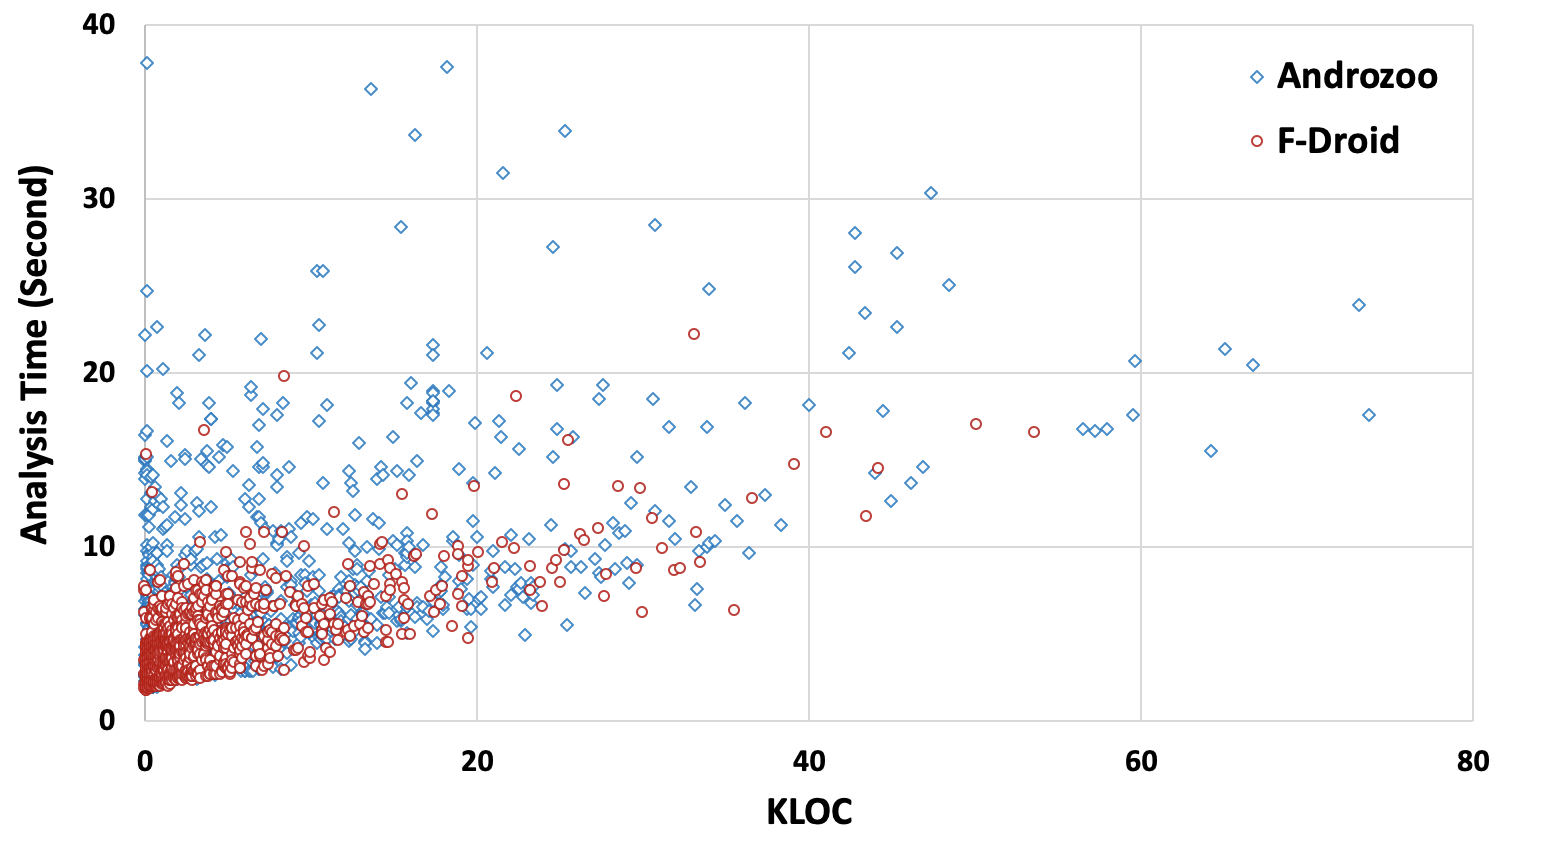
\includegraphics[width=0.46\textwidth]{images/scatterplot.png}
    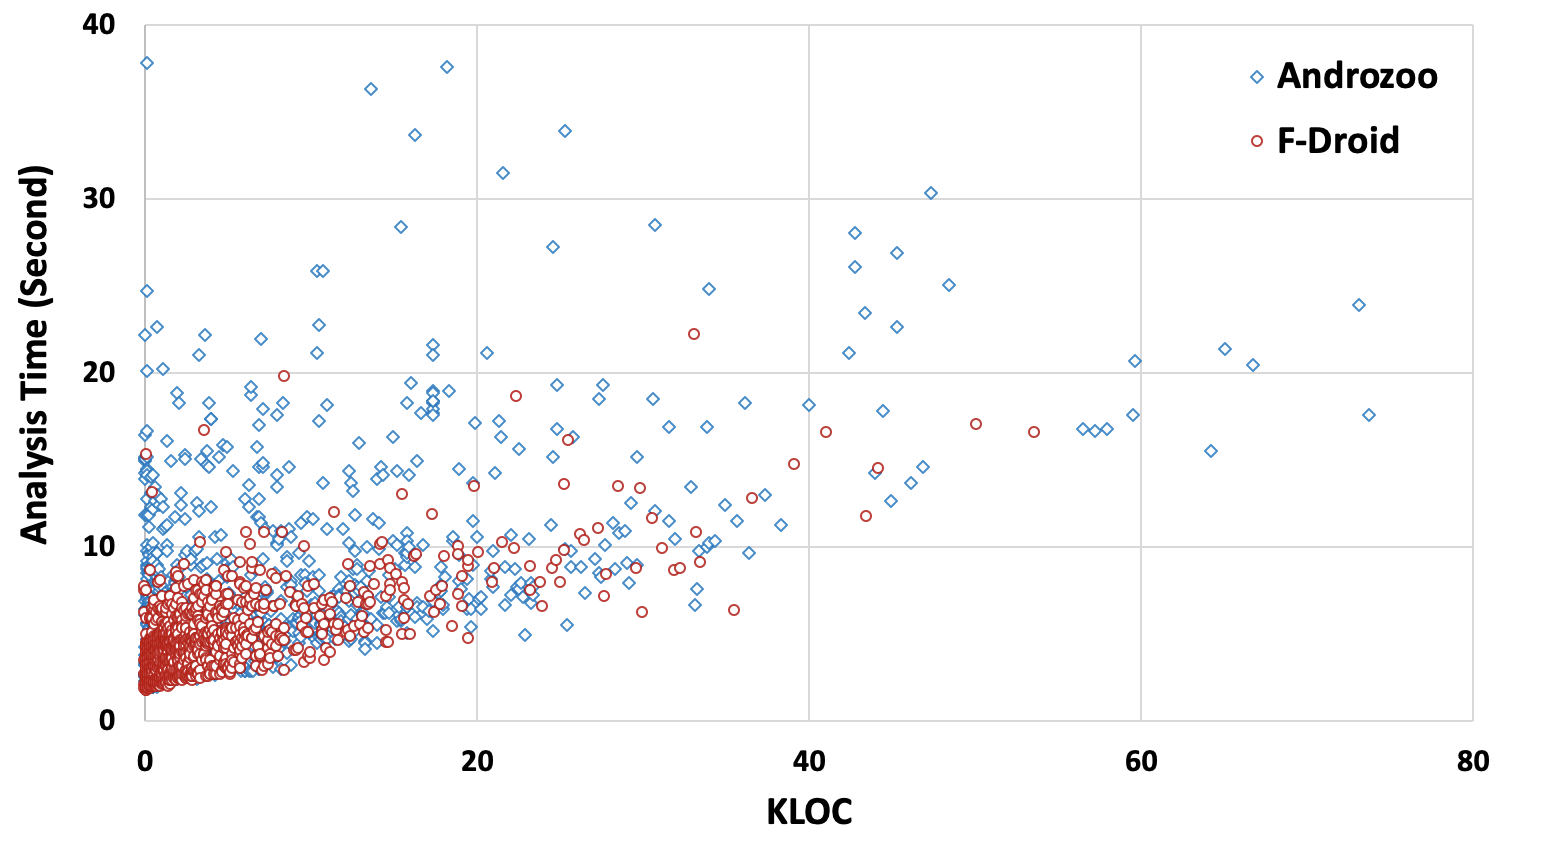
\includegraphics[width=\linewidth]{images/scatterplot.png}
    \caption{Scatter plot representing analysis time for compatibility checking of Android apps using \@approach.}
    \label{fig:scatterplot}
\end{figure}


\subsection{RQ3: Performance} % and Timing}

Table~\ref{tab:tab-timing-results} shows the analysis
times of \@approach, {\sc CiD}, and {\sc Lint} (in
seconds).  Dashes indicate that either the
corresponding technique fails to produce analysis
results after 600 seconds or crashes.
%timeouts.  after 10 minutes of analysis.
As shown, the analysis time taken by \@approach is
significantly lower than those of \textsc{CiD} and
\textsc{Lint} for almost all the apps. Also note that
\textsc{CiD} fails to completely analyze four apps.
Figure~\ref{fig:scatterplot} presents the time taken by
\@approach to perform compatibility analysis on
real-world apps.  The scatter plot depicts both the
analysis time and the app size.  The experimental
results show that the average analysis time taken by
\@approach, {\sc CiD}, and {\sc Lint} per app on
real-world data sets is 6.2 seconds (ranging from 1.6
to 37.8 seconds), 29.5 seconds (ranging from 4.1 to
78.4 seconds), and 24.7 seconds (ranging from 4.7 to
75.6 seconds), respectively. We have found outliers
during the analysis. For example, the app in the top
left corner in Figure~\ref{fig:scatterplot} is a game
application which extensively uses third party
libraries, which took a considerable amount of time for
the analyzer to compute the data structures required
for the compatibility analysis, despite its small KLOC.
On the other hand, the app in the right side of the
diagram, closer to 80 KLOC, loads three times less
library classes than the aforementioned app,
implicating in less complex graphs to analyze.
Overall, the timing results show that \@approach  is up
to 8.3 times (4.7 times on average) faster than the
state-of-the art techniques, and is able to complete
analysis of real-world apps in just a few seconds (on
an ordinary laptop), confirming that the presented
technology is indeed feasible in practice for
real-world usage.


\begin{figure}[b!]
	\centering
%	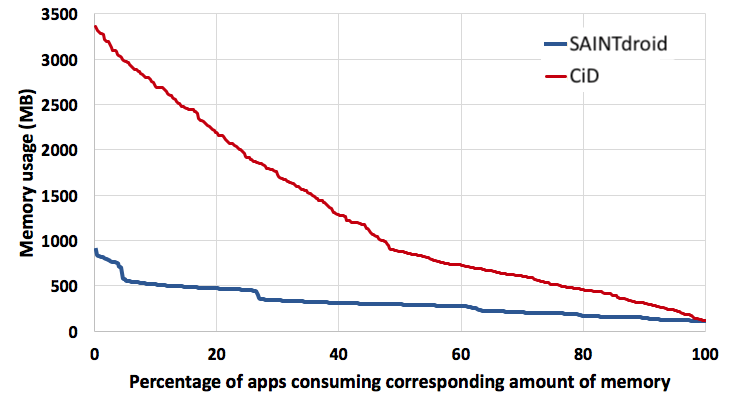
\includegraphics[width=0.42\textwidth]{images/memory_gd.png}
	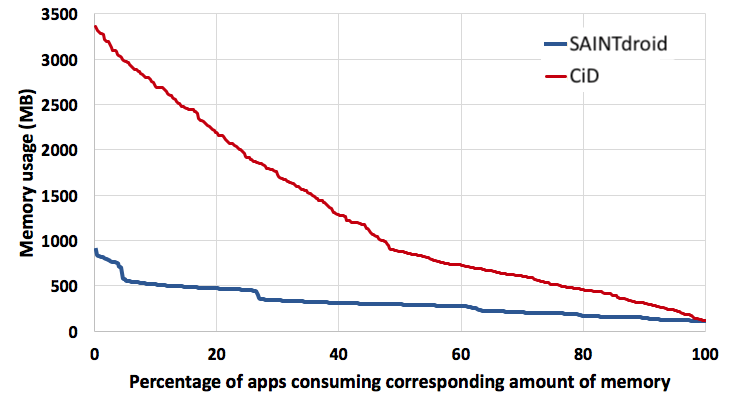
\includegraphics[width=\linewidth]{images/memory_gd.png}
	\caption{Amount of memory used by \@approach and \textsc{CiD} when analyzing real-world Android apps.}
	\label{fig:memory_gd}
\end{figure}

To better understand why \@approach performs more efficient than the state-of-the-art approaches, we conducted further performance evaluation, comparing the amount of
resources and analysis efforts required by each approach. 
\begin{comment}
%Our approach extends a class-loader based program analysis framework while {\sc CiD} is based on {\sc Soot}, which is a compiler based program analysis framework. \textcolor{blue}{To start the performance comparison, we monitored the number of analyzed classes in each approach.}
Since our approach extends a class-loader based program analysis framework rather than a compiler based program analyzer, %---e.g., {\sc CiD} is based on the {\sc Soot} framework---
we expect the efficiency gains in \@approach is due to the effective loading of classes during the analysis. In this set of experiments, we attempted to corroborate our intuition and obtain empirical evidence of this relationship.




We first monitored the number of analyzed classes in each approach.
%We notice that {\sc CiD} needs to load all of the Android classes prior to performing its analysis. On the contrary, \@approach only loads the classes that the app actually uses. 
Figure~\ref{fig:classes_loaded} depicts the number of classes loaded by \@approach and \textsc{CiD} when analyzing real-world apps.
The red line in Figure~\ref{fig:classes_loaded} shows that {\sc CiD} loads all Android classes from the latest available Android framework ~\cite{AndroidAOSP}. 
As of January 2019, there are 8552 classes in the Android framework. 
On the contrary, \@approach only loads the classes that the app actually uses. 
According to the diagram, \@approach, shown by the blue line in Figure~\ref{fig:classes_loaded}, at most loads 3,600 classes, and that only occurs for a very small number of apps. 
Indeed, for over 60\% of the analyzed apps, \@approach loads less than 1,000 classes , which is eight times more efficient compared to \textsc{CiD}. 
%For around 20\% of all real-world apps, \@approach loads just above 2,000 classes (shown by the blue line in Figure~\ref{fig:classes_loaded}). It is also interesting to note that for analyzing 60\% of the apps, \@approach loads less than 1,000 classes, which is 8 times more efficient compared to \textsc{CiD}.

 
%Loading fewer classes also allows \@approach to require less memory to perform its analysis. To investigate this matter, we also monitored the memory footprint required by each approach for performing analysis. Figure~\ref{fig:memory} shows a comparison of how much memory \@approach, {\sc CiD} and {\sc Lint} are using during the analysis of benchmark apps. According to the results, \@approach on average requires 265 MB of memory to perform compatibility analysis, which is by and large similar to what {\sc Lint} requires. {\sc CiD}, on the other hand, needs 1.3 GB (or five times more memory) to perform the same analysis. We have also observed \@approach's memory usage behavior while analyzing a set of real-world apps. As shown in Figure~\ref{fig:memory_gd}, \@approach on average  requires 329 MB (ranging from 898MB to 110MB) to analyze real-world Android apps, corroborating  the effectiveness of the our technique based on a class-loader based approach for compatibility analysis.

Loading fewer classes also allows \@approach to require less memory to perform its analysis. To investigate this matter, we also 
\end{comment}
Specifically, we monitored the memory footprint
required by each approach for performing analysis.
Figure~\ref{fig:memory_gd} shows a comparison of how
much memory \@approach and {\sc CiD} are using during
the analysis of real-world apps. According to the
results, \@approach on average requires 329 MB (ranging
from 119MB to 898MB) of memory to perform the
compatibility analysis. On the other hand, {\sc CiD} on
average uses 1.3 GB (or four times more memory) to
perform the same analysis.  We interpret this data as
corroborating the effectiveness of our compatibility analysis in
practice.



%\vspace{-0.2cm}
\section{Discussion}\label{sec-discussion}

%Next we discuss 
%This section discusses the limitations of \@approach. 
Like any approach relying on static analysis, \@approach is subject
to false positives. A promising avenue of future research is
to complement \@approach with dynamic analysis techniques.
Essentially, it should be possible to utilize dynamic
analysis techniques to automatically verify
incompatibilities identified through our conservative,
static analysis based, incompatibility detection technique,
further alleviating the burden of manual analysis.

As explained in Section~\ref{sec-results}, the majority of the
false alarms are due to a limitation in \@approach regarding
dynamically-generated classes (e.g., {\sf WebView\$1}) that
correspond to anonymous inner class declarations.  When
analyzing the code of each app, \@approach only explores the
explicit classes defined in the app, ignoring the
dynamically-generated classes. Thus, any callback or method
defined inside an anonymous inner class is invisible to
\@approach and is not included in the analysis. We plan to
address this limitation in the future by including the
dynamically-generated class definitions as well.


\begin{comment}
%\commentcs{

During development, we also encountered a false negative in
\emph{Padland}~\cite{padland}.  Huang et al. reported that
there is a callback API incompatibility in this app. There
is also a bug report on it. However, \@approach did not
initially detect any incompatibility issue. We then manually
inspected the call-graph generated by \textsc{Jitana}.
Again, we found no such incompatible API call in the graph.
This clearly explained why no issue was detected. Further
inspection, however, revealed that \emph{Padland} employs
two Dex files, and \@approach only analyzed the main Dex
file; however, the incompatibility is in the second Dex
file. We then reconfigured \@approach to analyze information
of all Dex files in an app and we were able to detect this
incompatibility.

%}

\commentcs{
We initially anticipated that apps that have been
specified to support wider ranges of API levels would
likely encountered more API incompatibility issues.
However, the experimental result clearly indicates that
such a correlation does not exist. The two apps with
most detected incompatibility issues support the ranges
of 10 (\emph{MaterialFBook}) and 8 (\emph{AFWall}) API
levels, respectively.  On the other hand, the two apps
that support the widest ranges of API level (15 for
\emph{SurvivalManual} and 14 for \emph{Simple
Solitaire}) only show 0 and 1 incompatibility issues,
respectively.
}

%As mentioned in Section~\ref{sec-eval}, \@approach reported
%a few number of false positives and negatives. The false
%positives identified in the {\it KolabNotes} app stem from
%its use of an external Java library, the methods of which
%GAINDroid incorrectly interpreted as API methods, resulting
%in false positives when those methods did not appear in the
%API database. Another false positive, in {\it
%SimpleSolitaire}, is due to a mistaken decoding of a call
%to {\sf Checkable.setChecked} (API 1) as a call to {\sf
%TwoStatePreference.setChecked} (API 14).

%The remaining errors---all five false negatives and one false positive---are due to a limitation in \@approach regarding anonymous inner classes. When analyzing the code of each app, \@approach only explores the explicit classes defined in the app, ignoring the dynamically-generated classes (e.g., {\sf WebView\$1}) that correspond to anonymous inner class declarations. Thus, any callback or method defined inside an anonymous inner class is invisible to \@approach and is not included in the analysis, resulting in the false negatives and the remaining false positive. We plan to address this limitation in the future by including the dynamically-generated class definitions as well.

Looking forward, as Android continues to add and deprecate
APIs as part of platform evolution, we also need to update
the database used by \@approach.  Such evolution may also
require that apps be reanalyzed to ensure API compatibility.
Because \@approach can perform analysis efficiently,
re-analyzing apps should only be quite feasible due to small
analysis time.

\commentcs{Android is trying to decrease API and permission
incompatibilities by enforcing new development rules. Google
Play recently required that new apps target at least Android
API level 26 and app updates target Android API level
26~\cite{googleIncomp} and Android 9 (API level 28)
introduced a new restriction regarding the use of hidden
APIs~\cite{googleHidden}.  Apps uploaded to other
repositories such as \cite{fdroid} and \cite{bazaar} could
still present runtime failures.}

\end{comment}

\section{Related Work}\label{sec-related}
%\vspace{-0.1cm}
%Android incompatibility issues have received a lot of
%attention recently. Here, we provide a discussion of the
%related efforts in light of our research.

\textbf{API evolution}. A large body of existing
research focuses on the evolving nature of APIs, which
is an important aspect of software
maintenance~\cite{mcdonnell2013empirical},
\cite{bavota2015impact}, \cite{ACRYL_Scalabrino2019},
\cite{li2018characterising},
\cite{lamothe2018exploring}, \cite{linares2013api},
\cite{Luo2018},
\cite{Fazzini:2017:ACI:3155562.3155604},
\cite{mahmoudi2018android}, \cite{mutchler2016target}.
These research efforts explore problems due to API
changes. Among others, McDonnell et
al.~\cite{mcdonnell2013empirical} studied Android's
fast API evolution (115 API updates/month), and noticed
developers' hesitation in embracing the fast-evolving
APIs because they can be more defect-prone than other
types of changes, which might cause application
instability and potential
vulnerabilities~\cite{linares2013api}.  
Bavota et al.  \cite{bavota2015impact}
showed that applications with higher user ratings use
APIs that are less change- and fault-prone compared to
the applications with lower ratings. 
%Mutchler et al.~\cite{mutchler2016target} explored the consequences
%of running applications targeted to older Android
%versions on devices with recent Android versions,
%and how it can introduce serious security issues. 
Li et al.  \cite{li2018characterising} investigated the
frequency with which deprecated APIs are used in the
development of Android apps, considering the deprecated
APIs' annotations, documentations, and removal
consequences along with developers' reactions to APIs
deprecations. 
%
%
%
%\textcolor{red}{
%The results of these studies, identifying potential issues
%caused by API evolutions, are the primary motivations for
%this work.
%
These prior efforts clearly motivate the need to address
issues relating to API evolution.  However, their
approaches do not provide detailed technical solutions or
methods to systematically detect the root causes of these
problems.  \textsc{\@approach}, on the other hand, is
designed to be effective at detecting crash-leading API
related issues.

%}

\begin{comment}

\textbf{Android testing}. The other line of related research
efforts involves techniques that have been proposed to
expose potential runtime errors, mainly using various
testing methods ~\cite{moran2016automatically},
\cite{khan2018crashsafe}, \cite{moran2017crashscope},
\cite{gomez2013reran}, \cite{amalfitano2012using},
\cite{amalfitano2015mobiguitar}. For example, Moran et al.
\cite{moran2017crashscope} presented a systematic input
generation driven by both static and dynamic analyses to
trigger app crashes. 
%Automatically discovering, reporting and reproducing
%android application crashes
Given such automatically generated inputs, it produces a
crash report containing screenshots, detailed crash
reproduction steps, the captured exception stack trace, and
a fully replayable script that automatically reproduces the
crash on a target device. Amalfitano et al.
\cite{amalfitano2015mobiguitar} extracted relationships
between GUI widgets to automatically generate test cases,
with the goal of yielding possible runtime errors raised by
the automatic generated test cases.
\textcolor{pblue}{However, testing by itself cannot uncover
the underlying reasons for application crashes. These
techniques generate inputs for the target app to exercise
illegal sequences of events that may lead to a crash. In
these works, detection of incompatible Android APIs across
different levels of the framework is missing. \@approach
however, addresses and detects this problem in Android
framework, which exists due to its fast paced API
evolution.}



\textbf{Android fragmentation}.  The other relevant thrust
of research has focused on investigating the Android
ecosystem by running different custom Android distributions
on different hardware to identify potential application
instability and uncovering the causes
\cite{han2012understanding}, \cite{li2015characterizing},
\cite{pathak2011bootstrapping},
\cite{liu2014characterizing}, \cite{zhou2014peril},
\cite{wei2016taming}, \cite{aafer2016harvesting}.  Aafer et
al. \cite{aafer2016harvesting} investigated how modifying
the operating system can introduce security problems within
the mobile OS. Han et al. \cite{han2012understanding}
studied the bug reports related to HTC and Motorola devices
in the Android issue tracking system, and discovered that
Android ecosystem was fragmented, meaning that applications
might behave differently when installed on phones from
different vendors. Liu et al. \cite{liu2014characterizing}
observed that a noticeable percentage of Android performance
bugs occur only on specific devices and platforms.  Moran et
al. \cite{moran2017crashscope} presented a systematic input
generation driven by both static and dynamic analyses to
trigger app crashes. 
%Automatically discovering, reporting and reproducing
%android application crashes
Given such automatically generated inputs, it produces a
crash report containing screenshots, detailed crash
reproduction steps, the captured exception stack trace, and
a fully replayable script that automatically reproduces the
crash on a target device.  
%
%\textcolor{red}{

These research efforts primarily focused on
behavioral differences when an app is installed on different
operating systems and/or hardware platforms.  They mainly
rely on hardware specifications and changes in the Android
documentation to uncover potential compatibility or
behavioral issues. Therefore, these approaches are not
useful when such platform related information is incomplete,
inconsistent, or unavailable.  Furthermore,  applying these
approaches to test an application on the entire vast
hardware ecosystem of Android devices may not be feasible
due to exponentially large system configurations.  Our work,
on the other hand, focuses on a more tractable and important
problem due to API evolution and how it can affect the apps
and their performance regardless of the operating system
distribution or the hardware the applications are running
on.

\end{comment}

\textbf{API incompatibility}. 
In Table~\ref{tab:table_comparison_tools}, we compare the
detection capabilities of \textsc{\@approach} against the
current state-of-the-art approaches. It is important to
stress that \@approach is the only solution that 
can automatically detect API invocation
compatibility issues (API), API callback compatibility
issues (APC), and permission-induced compatibility issues
(PRM). %We continue to discuss some of the closely related works to ours and the differences between those works and ours.
%compared to the one issue identified by each of the other
%approaches.

\begin{table}%{R}{0.40\textwidth}
    %\vspace{-5ex}
    %\begin{table}
\centering
\caption {Comparing \@approach to the state-of-the-art of compatibility detection techniques.} %, \@approach is the only solution that provides  
%\vspace{-0.2cm}
%\scriptsize{
\footnotesize{
%\small{
\begin{tabular}{l|c|c|c} 
    \hline
    \hline    
    \rule{0pt}{3ex}
    & API & APC & PRM     \\ 
    \hline \hline
   \rule{-3pt}{3ex}
    \textsc{CiD}~\cite{lili2018cid}              & $\cmark$ & $\xmark$ & $\xmark$\\
    \textsc{Cider}~\cite{huang2018understanding} & $\xmark$ & $\cmark$ & $\xmark$\\
    IctApiFinder~\cite{he2018understanding} 		& $\cmark$ & $\xmark$ & $\xmark$\\    
    \textsc{Lint}~\cite{linttips}                & $\cmark$ & $\xmark$ & $\xmark$\\
    \textsc{\@approach}                 & $\cmark$ & $\cmark$ & $\cmark$ \\
    \hline
    \hline
\end{tabular}
%\vspace{-0.2cm}
}

\label{tab:table_comparison_tools}
%\end{table}

    \vspace{-0.5cm}
\end{table}

Wu et al.~\cite{wu2017measuring} investigated side
effects that may cause runtime crashes even within an
app's supported API ranges, inspiring subsequent work.
%
Huang et al.~\cite{huang2018understanding} aimed to
understand callback evolution and developed
\textsc{Cider}, a tool capable of identifying API
callback compatibility issues. However,
\textsc{Cider}'s analysis relies on manually built
PI-GRAPHS, which are models of common compatibility
callbacks of four classes: Activity, Fragment, Service
and WebView. \textsc{Cider} thus does not deal with
APIs that are not related to these classes or
permission induced mismatches. 
%As this tool focuses on these predefined callback
%classes, Moreover, by only focusing on callback
%classes, 
As such, their reported result is a subset of ours. In
addition, \textsc{Cider}'s API analysis is based on the
Android documentation, which is known to be
incomplete~\cite{wu2017measuring}. Our work, on the
other hand, automatically analyzes each API level in
its entirety to identify all existing APIs. This allows
our approach to be more accurate in detecting actual
changes in API levels, as there are frequent platform
updates and bug fixes. As a result, and as confirmed by
the evaluation results, our approach features much
higher precision and recall in detecting compatibility
issues.
%\textsc{Cider} also relies on constructing Callback
%Control Flow Graph, while our analysis simply works on
%an existing method call graph and data flow graphs
%generated by \textsc{Jitana} to help us uncover
%sources of potential issues.}  % but it comes at a
%cost of higher manual efforts and possibly longer
%analysis time. However, while being able to complete
%each analysis in just a few seconds.  Another
%difference between the two approaches is that their
%analysis is based on \textsc{Soot}, which requires the
%Dex code be converted to Jimple.

Lint \cite{linttips} is a static analysis tool
introduced in ADT (Android Development Tools) version
16. One of the benefits of Lint is that the plugin is
integrated with the Android Studio IDE, which is the
default editor for Android development. The tool checks
the source code to identify potential bugs such as
layout performance issues, and accessing API calls that
are not supported by the target API version. However,
the tool generates false positives when verifying
unsupported API calls (e.g., when an API call happens
within a function triggered by a conditional
statement). Another disadvantage is that it requires
the availability of the original Java source code, and
it does not analyze APKs.  In addition, \textsc{Lint}
requires the project to be first built in the Android
Studio IDE before conducting the analysis.  Unlike
\textsc{Lint}, \@approach operates directly on Dex
code. While \textsc{Lint} claims to be able to detect
API incompatibility issues, our experimental results as
well as the results obtained by Huang et al.  indicate
that \textsc{Lint} is not as effective as \@approach. %or \textsc{Cider}.

Li et al.~\cite{lili2018cid} provided an overview of the
Android API evolution to identify cases where compatibility
issues may arise in Android apps. They also presented
\textsc{CiD}, an approach for identifying compatibility
issues for Android apps. This tool models the API lifecycle,
uses static analysis to detect APIs within the app's code,
and then extracts API methods from the Android framework to
detect backward incompatibilities.  \textsc{CiD} supports
compatibility analysis upto the API level 25.  In
comparison, \@approach offers automated extraction of the
API database, and thereby supports up to the most recent
Android platform (API level 29).  Moreover, in contrast to
\@approach, \textsc{CiD} did not consider incompatibilities
regarding the runtime permission system.

Wei et al.~\cite{wei2016taming} conducted a study to
characterize the symptoms and root causes of compatibility
problems, concluding that the API evolution and problematic
hardware implementations are major causes of compatibility
issues. They also propose a static analysis tool to detect
issues when invoking Android APIs on different devices.
Their tool, however, needs manual work to build API/context
pairs, of which they only define 25. Similar to our prior
discussion of work by Huang et al., the major difference
between our work and this work is that our approach can
focus on all API methods that exist in an API level. Again,
the result reported by their approach would be a subset of
our detected issues.

%\vspace{-0.3cm}
\section{Conclusion and Future Work}\label{sec-conclusion}
%\vspace{-0.1cm}

This paper presents \@approach, a novel approach and
accompanying tool-suite for efficient analysis of various
types of crash-leading Android compatibility issues.  The
experimental results of comparing \@approach with the
state-of-the-art in Android incompatibility detection
corroborate its ability to efficiently detect more sources
of potential issues, yielding fewer false positives and
executing in a fraction of the time needed by the other
techniques.  Applying \@approach to thousands of real-world
apps from various repositories reveals that as many as 42\%
of the analyzed apps are prone to API invocation mismatch,
20\% can crash due to API callback mismatch, and 40\% of the
apps can suffer from crashes due to permissions-related
mismatch, indicating that such problems are still prolific
in contemporary, real-world Android apps. 
%and that
%\@approach can successfully perform large scale analysis.

Besides what we already discussed in Section~\ref{sec-discussion}, we also plan as part of our future work to explore the trade-off between increasing analysis precision, e.g.,
through incorporating additional information such as CCFG for the compatibility analysis, and higher analysis overhead. In addition, we plan to develop a complementing code synthesizer to help repair apps that do not properly handle detected mismatches. 

\begin{comment}
\commentcs{
We also plan to develop new detectors to identify other events that can lead to dependability and security issues. 
Another idea
is to provide guidance to users to replace the use of
possibly outdated or deprecated APIs with more updated
ones.  For example, our system can recommend a
developer to replace the old SSL API with the new one.
While the old one still works,  it is less secure than
the newer API.
}
\end{comment}
 

 
%\@approach will be made available to other researchers and practitioners upon the publication of this work.


%\newpage
%\balance
%\bibliographystyle{ACM-Reference-Format}
\bibliographystyle{IEEEtran}
\bibliography{paper}

\end{document}


 
